 %------------------------------------------------------------------------------
% Template file for the submission of papers to IUCr journals in LaTeX2e
% using the iucr document class
% Copyright 1999-2013 International Union of Crystallography
% Version 1.6 (28 March 2013)
%------------------------------------------------------------------------------

\documentclass[preprint]{iucr}       % DO NOT DELETE % 
\usepackage{bm}
% \usepackage{graphicx}
% \usepackage{tabularx}
% \usepackage{subfigure}
% \usepackage{afterpage}
% \usepackage{sansmath}
\usepackage{mathtools}
% \usepackage{parskip}
\usepackage{tikz}
% \usepackage{tikzorbital}
% \usepackage{setspace}
% \usepackage{xcolor}
% \usepackage{amssymb}
% \usepackage{bm}
\usepackage{amsmath}
% \usepackage{fancyhdr}
% \usepackage{rotating}
\usepackage{siunitx}
\usepackage[hyphens,spaces,obeyspaces]{url}
\usepackage{color}
\usepackage{cprotect}
\usepackage{textgreek}
\usepackage[normalem]{ulem}
\usepackage{hyperref}

\newcommand{\todo}[1]{{\color{red}[TODO: "#1'']}}
\newcommand{\inblue}[1]{{\color{blue}#1}}
\newcommand{\inred}[1]{{\color{red}#1}}
\newcommand{\ingreen}[1]{{\color{green}#1}}



   %-------------------------------------------------------------------------
   % Infobrmation about journal to which submitted
   %-------------------------------------------------------------------------
   \journalcode{S}       % Indicate the journal to which submitted
                 %  A - Acta Crystallographica Section A
                 %  B - Acta Crystallographica Section B
                 %  C - Acta Crystallographica Section C
                 %  D - Acta Crystallographica Section D
                 %  E - Acta Crystallographica Section E
                 %  F - Acta Crystallographica Section F
                 %  J - Journal of Applied Crystallography
                 %  M - IUCrJ
                 %  S - Journal of Synchrotron Radiation

\begin{document} % DO NOT DELETE THIS LINE

   %-------------------------------------------------------------------------
   % The introductory (header) part of the paper
   %-------------------------------------------------------------------------

   % The title of the paper. Use \shorttitle to indicate an abbreviated title
   % for use in running heads (you will need to uncomment it).


\title{Simulations of applications using diaboloid mirrors}

\cauthor[a,b]{Manuel}{Sanchez del Rio}{srio@esrf.eu}{address if different from \aff}
\author[a]{Kenneth A.}{Goldberg}
\author[a]{Valeriy V.}{Yashchuk}
\author[a]{Ian}{Lacey}
\author[a]{Howard A.}{Padmore}

\aff[a]{Advanced Light Source, LBNL, Berkeley CA, \country{USA}}
\aff[b]{European Synchrotron Radiation Facility, 71 Avenue des Martyrs F-38000 Grenoble \country{France}}



\begin{synopsis}
The diaboloid mirror is a surface that converts a spherical wave to a cylindrical wave. It finds application in beanding-magnet beamlines at low-emittance storage rings, such as ALS-U. We model diaboloid mirrors and study by ray tracing the benefit of using this mirror.
\end{synopsis}

\begin{abstract}
The diaboloid is a reflecting surface that converts a spherical wave to a cylindrical wave. This complex surface may find application in new Advanced Light Source bending magnet beamlines or in other beamlines that now use toroidal optics for astigmatic focusing. We describe here the numerical implementation of the diaboloid mirrors and study by ray tracing the benefit of this mirror in beamlines exploiting diffraction-limited storage rings.
\inred{The use of diaboloids becomes especially interesting for the new low-emittance storage rings because for such small sources the reduction of aberration becomes essential. The validity of the toroidal and other mirror surfaces approximating the diaboloid, and the effect of the mirror magnification are discussed.}
\end{abstract}

\section{Introduction}

In the development of synchrotron radiation sources, brightness has always been a key metric, and as such the strongest emphasis is on insertion device performance. Bending magnet development has been a secondary consideration, yet these white light sources hold important advantages for a range of x-ray experiments, such as Laue diffraction, energy-dispersive EXAFS (Extended X-ray Absorption Fine Structure) and other experiments that take advantage of a wide energy spectrum. In other areas, the agility in photon energy offered by monochromatized bending magnet radiation is a great advantage. 

Now, with the advent of 4\textsuperscript{th} generation multi-bend achromat (MBA) synchrotrons with smaller electron beam widths, bending magnet sources are becoming even more attractive for a segment of synchrotron experiments. However, a technical challenge is preserving the brightness while imaging a significant horizontal aperture. With shrinking source sizes, preserving the source brightness requires a reduction in the range of tolerable shape and slope errors: new shape optimizations need to be found. Advances in aspheric mirror fabrication and metrology increase the breadth and feasibility of potential solutions.

With undulator sources and their narrow divergence angles, we have the luxury of using only tangentially curved optics for focusing in both horizontal and vertical planes. However for bending magnet sources, with their wide horizontal fan, to collect a reasonable aperture, we have to use sagittaly curved optics. This could be as in a crystal monochromator with a sagittaly curved 2\textsuperscript{nd} crystal, or with a sagitally focusing cylindrical or toroidal mirror.

At the Advanced Light Source (ALS), we adopted toroidal mirrors for protein crystallography beamlines, due to the robustness of the optical system. We found that a specific configuration \inred{with two mirrors and a monochromator in between, all deflecting  the vertical plane,} could preserve brightness and eliminate coma aberrations. 
A tangentially collimating pre-mirror \inred{assures negigible vertical divergence at the monochromator entrance, thus optimizing its energy resolution,} and a toroidal mirror downstream of the crystal monochromator \inred{refocuses the beam at the focal plane.} The optimal design focuses from infinity in the vertical direction and from the real source in the horizontal direction with a 1:2 magnification.

This arrangement was used in ALS \emph{superbend} beamlines, as originally described by MacDowell \cite{MacDowell2004}. At the time, the horizontal source size was \SI{100}{\micro\meter} root mean square (RMS) and the residual aberrations in the image produced by a toroidal mirror were far less. Following an upgrade of the ALS in 2013, the horizontal photon beam size was reduced \cite{Steier_2014} to \SI{26}{\micro\meter} RMS. The residual aberrations were tolerable, but cause a factor of two decrease in brightness. The ALS upgrade project, now in progress, will reduce the horizontal beam size to
% \inred{\sout{7}}
\SI{10}{\micro\meter} RMS. At this size, the residual aberrations of optical systems based on toroids will no longer be acceptable, and new types of brightness-preserving optics are required.

For many applications we need good monochromatization and tunability, such as is provided by the classical, collimated double crystal monochromator. To preserve the source brightness, the task is therefore to design a single optical element that can accept light from infinity in the vertical direction (i.e. vertically collimated) and from the real source in the horizontal direction, and focus that light to a point, unifying two properties not found in a single canonical shape.
%Because a parabolic surface can provide vertical collimation of a point source in one direction, the central vertical cross-section (i.e. the tangential shape) of the mirror will be parabolic. Ellipsoidal surfaces provide point-to-point focusing for rays outside of this central plane of incidence. Therefore, sagittal cross-sections will be elliptical.
Because a parabolic surface can provide vertical collimation of a point source in one direction, the central vertical cross-section (i.e. the tangential shape) of the mirror will be parabolic. The sagittal curvature provide point-to-point focusing for rays outside of this central plane of incidence.

Such a surface was first described by McKinney \cite{McKinneySPIE2009} and named the \emph{diaboloid}, to indicate the probable difficulty in making this type of optical element. The surface was represented with a polynomial series, derived from classical optical path function analysis. This work showed the expected, optimal focusing properties and the benefits for small, high brightness beams with a large horizontal fan angle. McKinney {\it et al.} also showed that at 1:2 magnification, a toroidal mirror comes closest to the ideal diaboloid shape, minimizing, although not eliminating, residual aberrations.

Although the idea is to replace the toroidal mirrors in ALS protein crystallography, superbend beamlines with this new type of mirror, the application goes further than this: the diaboloid allows us to demagnify more strongly than before. One such example is in a high-pressure-science beamline currently using a 1:2 magnification toroidal mirror, further demagnified to a few-micron focus using a Kirkpatrick-Baez (K-B) mirror pair \cite{Kirkpatrick1946}. In an updated, diaboloid-based optical system, the K-B mirrors become unnecessary and the single diaboloid mirror will focus directly to approximately \SI{3}{\micro\meter} spot size, increasing flux and image quality while decreasing complexity.

It is important to note that until recently, the fabrication of such complex surfaces has not been been possible at the error levels that we require. For a typical application at the \inred{upgraded} ALS, the mirror-to-source distance is \SI{20}{\meter}\inred{, the mirror-to-focal plane is \SI{10}{\meter} (magnification 1:2)}, and so with a \SI{7}{\micro\meter} vertical source size \inred{RMS}, including angle doubling on reflection, the tangential slope error tolerance is \SI{0.17}{\micro\radian} \inred{RMS.}. The sagittal slope error tolerance is \SI{34}{\micro\radian} \inred{due to the forgiveness factor}. The tangential tolerance is extremely challenging, but mainly limited by metrology. Local area correction, and stitching-interferometer-based metrology have led to the creation of 1D curved optics with significantly smaller slope errors \cite{Yamauchi2002}. 
%The problem is that current high accuracy metrology techniques cannot accommodate steeply curved optics. One possible solution is to use metrology based on computer generated hologram (CGH) reference beams, as now widely used in free form optics fabrication.
A difficulty is the availability of high accuracy metrology to measure steeply curved optics. One possible solution is to use metrology based on computer generated hologram (CGH) \inred{\cite{Wyant, Poleshchuk}} reference beams, as now widely used in free form optics fabrication. 
\inred{Recent progress in metrology techniques \cite{diamond2019} also supported by international collaborations, e.g.,  Europe’s MooNpics, are actively working to improve high-accuracy figure error measurements on a variety of surfaces. 
}
Advances in fabrication and metrology make these optics feasible now.


In Section \ref{sec:approximatedShapes}, we investigate various approximations to the diaboloid which may be easier to manufacture.

In the 1:2 magnification case, the deviation of the diaboloid surface from a toroid is approximately \SI{2}{\micro\meter} for the extreme sagittal positions
\footnote{\inred{this is valid for a grazing angle $\theta$~= \SI{2}{\milli\radian} on a \SI{10}{\milli\meter} wide mirror of length \SI{200}{\milli\meter} as it will be seen in Fig.~\ref{fig:detrendedBeamline}a. If the diaboloid is approximated by a cone (Fig.~\ref{fig:detrendedBeamline}b), or the grazing angle is increased (Fig.~\ref{fig:detrended}e), the difference of \SI{2}{\micro\meter} is valid over a mirror width of \SI{20}{\milli\meter} }}. Therefore, it may be possible to manufacture them using gradient deposition in the sagittal direction. As a toroid can be produced from a sagittal cylinder by bending, we know from experience that the tangential slope can achieve the error levels required.


To study diaboloid mirrors in beamline optical simulations, we created a tool in the Oasys environment \cite{codeOASYS} that implements diaboloid surfaces and their approximations \cite{valSPIE} \cite{val2021}. The new Oasys widget (Section~\ref{sec:oasys}) sends the created surface to the ray tracing code SHADOW \cite{codeSHADOW}. We used this application to make simulations of the ALS beamline 12.2.2 (Section~\ref{sec:beamline}) where the original toroid is replaced with a diaboloid and the performance is compared for the present ALS storage ring and for the future upgraded ALS. Section~\ref{sec:scan} investigates a possible upgrade of this beamline using high demagnification and analyzes the feasibility of using a simpler \emph{parabolic-cone} to replace diaboloids. The use of surfaces that approximate the diaboloid is analyzed in Section~\ref{sec:approximatedShapes}.

\section{Definition and implementation of the diaboloid surface}
\label{sec:DiaboloidEqs}

For practical purposes we want to define the diaboloid surface as a function of the focal distances, $p$ and $q$ ($p$ is the source-to-mirror distance, $q$ is the mirror-to-image distance), and the grazing incidence angle, $\theta$. The diaboloid can be placed in two configurations: i) ``collimating'' to convert a spherical wave into a cylindrical wave (geometrically, a point-to-line focusing, and ii) ``focusing'' to convert a cylindrical wave into a spherical one (or segment-to-point focusing). The latter (Fig.~\ref{fig:frame}) is the usual configuration in synchrotron beamlines, where the main purpose is to refocus a beam that is vertically collimated and horizontally diverging. 

%\tikzset{every picture/.style={line width=0.75pt}} %set default line width to 0.75pt    

\begin{figure}\label{fig:frame}
\includegraphics[width=0.95\textwidth]{figures/fig1.pdf}
%%\tikzset{every picture/.style={line width=0.75pt}} %set default line width to 0.75pt        

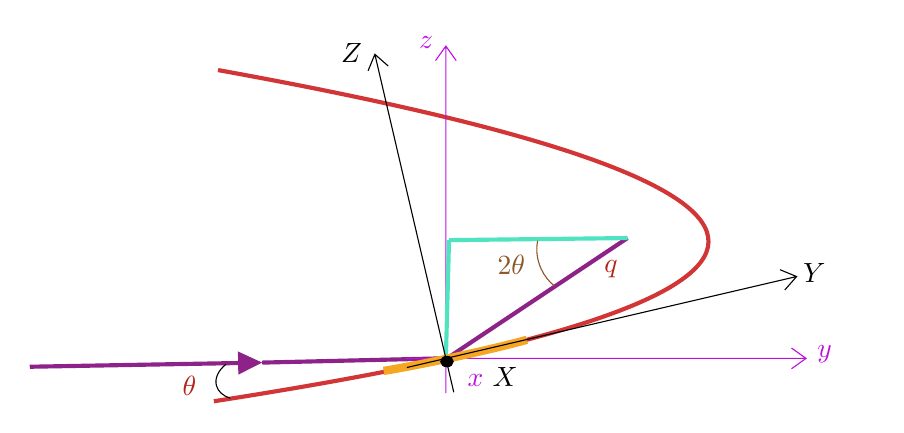
\begin{tikzpicture}[x=0.75pt,y=0.75pt,yscale=-1,xscale=1]
%uncomment if require: \path (0,214); %set diagram left start at 0, and has height of 214

%Shape: Parabola [id:dp636758281566334] 
\draw  [color={rgb, 255:red, 209; green, 53; blue, 53 }  ,draw opacity=1 ][line width=1.5]  (215.73,193.63) .. controls (532.78,144.36) and (533.44,91.17) .. (217.71,34.06) ;
%Straight Lines [id:da5751643928734858] 
\draw [color={rgb, 255:red, 141; green, 34; blue, 137 }  ,draw opacity=1 ][line width=1.5]    (239,175) -- (324,173) ;
%Straight Lines [id:da4985393188459284] 
\draw [color={rgb, 255:red, 141; green, 34; blue, 137 }  ,draw opacity=1 ][line width=1.5]    (328,173) -- (415,115) ;
%Shape: Axis 2D [id:dp5339485321600788] 
\draw [color={rgb, 255:red, 189; green, 16; blue, 224 }  ,draw opacity=1 ] (308.2,172.98) -- (501,172.98)(327.48,22.53) -- (327.48,189.7) (494,167.98) -- (501,172.98) -- (494,177.98) (322.48,29.53) -- (327.48,22.53) -- (332.48,29.53)  ;
%Straight Lines [id:da984423242776999] 
\draw [color={rgb, 255:red, 141; green, 34; blue, 137 }  ,draw opacity=1 ][line width=1.5]    (127,177) -- (235,175.07) ;
\draw [shift={(239,175)}, rotate = 538.98] [fill={rgb, 255:red, 141; green, 34; blue, 137 }  ,fill opacity=1 ][line width=0.08]  [draw opacity=0] (11.61,-5.58) -- (0,0) -- (11.61,5.58) -- cycle    ;
%Straight Lines [id:da25833218941129754] 
\draw [color={rgb, 255:red, 80; green, 227; blue, 194 }  ,draw opacity=1 ][line width=1.5]    (329,116) -- (415,115) ;
%Straight Lines [id:da4020633150416717] 
\draw [color={rgb, 255:red, 80; green, 227; blue, 194 }  ,draw opacity=1 ][line width=1.5]    (329,116) -- (327.48,172.98) ;
%Shape: Arc [id:dp507008334854385] 
\draw  [draw opacity=0] (379.83,138.12) .. controls (377.17,136.02) and (374.91,133.19) .. (373.35,129.77) .. controls (371.31,125.28) and (370.83,120.52) .. (371.71,116.28) -- (389.13,122.59) -- cycle ; \draw  [color={rgb, 255:red, 139; green, 87; blue, 42 }  ,draw opacity=1 ] (379.83,138.12) .. controls (377.17,136.02) and (374.91,133.19) .. (373.35,129.77) .. controls (371.31,125.28) and (370.83,120.52) .. (371.71,116.28) ;
%Shape: Arc [id:dp28668965321519213] 
\draw  [draw opacity=0] (223.6,192.18) .. controls (220.17,191.08) and (217.66,188.93) .. (216.92,186.03) .. controls (216.01,182.5) and (217.91,178.69) .. (221.55,175.8) -- (232.39,182.04) -- cycle ; \draw   (223.6,192.18) .. controls (220.17,191.08) and (217.66,188.93) .. (216.92,186.03) .. controls (216.01,182.5) and (217.91,178.69) .. (221.55,175.8) ;
%Curve Lines [id:da06756156046542072] 
\draw [color={rgb, 255:red, 245; green, 166; blue, 35 }  ,draw opacity=1 ][line width=3]    (297.5,179) .. controls (318.17,175.67) and (355.17,167.33) .. (366.5,164) ;
%Shape: Axis 2D [id:dp06708045637689208] 
\draw [color={rgb, 255:red, 0; green, 0; blue, 0 }  ,draw opacity=1 ] (308.7,177.37) -- (496.46,133.54)(293.28,26.46) -- (331.28,189.26) (488.5,130.26) -- (496.46,133.54) -- (490.78,140) (290,34.42) -- (293.28,26.46) -- (299.74,32.14)  ;
%Shape: Ellipse [id:dp8232202429248765] 
\draw  [fill={rgb, 255:red, 0; green, 0; blue, 0 }  ,fill opacity=1 ] (325,174.5) .. controls (325,173.12) and (326.34,172) .. (328,172) .. controls (329.66,172) and (331,173.12) .. (331,174.5) .. controls (331,175.88) and (329.66,177) .. (328,177) .. controls (326.34,177) and (325,175.88) .. (325,174.5) -- cycle ;

% Text Node
\draw (510,171) node  [color={rgb, 255:red, 179; green, 35; blue, 24 }  ,opacity=1 ,rotate=-359.63]  {$\textcolor[rgb]{0.74,0.06,0.88}{y}$};
% Text Node
\draw (318,21) node  [color={rgb, 255:red, 179; green, 35; blue, 24 }  ,opacity=1 ,rotate=-359.63]  {$\textcolor[rgb]{0.74,0.06,0.88}{z}$};
% Text Node
\draw (282,26) node  [color={rgb, 255:red, 179; green, 35; blue, 24 }  ,opacity=1 ,rotate=-359.63]  {$\textcolor[rgb]{0,0,0}{Z}$};
% Text Node
\draw (505,132) node  [color={rgb, 255:red, 179; green, 35; blue, 24 }  ,opacity=1 ,rotate=-359.63]  {$\textcolor[rgb]{0,0,0}{Y}$};
% Text Node
\draw (350,182) node  [color={rgb, 255:red, 179; green, 35; blue, 24 }  ,opacity=1 ,rotate=-359.63]  {$\textcolor[rgb]{0.74,0.06,0.88}{x} \ \textcolor[rgb]{0,0,0}{X}$};
% Text Node
\draw (407,130) node  [color={rgb, 255:red, 179; green, 35; blue, 24 }  ,opacity=1 ,rotate=-359.63]  {$q$};
% Text Node
\draw (204,186) node  [color={rgb, 255:red, 179; green, 35; blue, 24 }  ,opacity=1 ,rotate=-359.63]  {$\theta $};
% Text Node
\draw (359,128) node  [color={rgb, 255:red, 139; green, 87; blue, 42 }  ,opacity=1 ,rotate=-359.63]  {$2\theta $};


\end{tikzpicture}


\caption{Schematic (vertical section) of the reference frames: mirror-related $(X,Y,Z)$ used for numerical implementation, and mirror-canonical $(x,y,z)$ where the diaboloid shape takes the form of equation~(\ref{eqn:diaboloidV}). }
\end{figure}


The equation of the diaboloid in the ``collimating'' configuration is (see Appendix \ref{appendix:diaboloid})
\begin{multline}
\label{eqn:diaboloidV}
z(x,y) = q \sin2\theta - 
[ (q \sin{2\theta})^2 + 2p^2 + 2 p q~+\\
2 (p + q \cos{2\theta}) y - 2 (p+q) \sqrt{x^2 + (y + p)^2}) ]^{1/2}.
\end{multline}

The mirror height $z$ = 0 at the mirror center position $x, y = 0$, as expected. The tangential profile ($x=0$) is a parabola with focal length $ f = (1-\cos2\theta) q/2$. For small angles, ($\cos2\theta\approx 1 - 2\theta^2$) and $|y|\ll q$ gives $z\approx 2 \theta q + \theta y$ with slope in the center $dz/dy=\theta$. The sagittal section ($y=0$) can be approximated by an ellipse with semiaxes $b=q \sin2\theta$ and $a=b \sqrt{q /(p+q)}$ (see Appendix \ref{appendix:diaboloid}). 

For ray tracing calculations, it is convenient to obtain the numerical mesh as a function of a mirror-based coordinate system ($X,Y,Z$) (Fig.~\ref{fig:frame}). This system has the origin in the center of the mirror, the $Y$-axis tangent to the surface origin in the direction of the beam propagation, the $X$-axis tangent to the surface origin in the sagittal direction, and the $Z$-axis normal to the surface at the origin. In most practical cases for x-ray optics, the grazing incidence $\theta$ is small, therefore equation~(\ref{eqn:diaboloidV}) can be expressed in the $X,Y,Z$ frame by rotating the surface about the $X$-axis to achieve zero slope at the origin (i.e., detrending the plane $z_{\mathrm{plane}}=y \theta$). This is done numerically after evaluating the surface using equation~(\ref{eqn:diaboloidV}). The exact, explicit, expression of the diaboloid $Z(X,Y)$ can be obtained from the rotation of equation~(\ref{eqn:diaboloidV}) by an angle $\theta$ \cite{val2021}, resulting in a fourth-degree polynomial equation $F(X,Y,Z)=0$. The explicit equation is therefore obtained by solving this equation for any point in the $(X_i,Y_j)$ mesh.


The simplest approximation of the diaboloid is the toroid, defined by circular cross-sections with \inred{tangential} and sagittal radii at the origin, $R_t$ and $R_s$, respectively. These values are known from Coddington's equations for focusing mirrors:
\begin{equation}
\label{eqn:radii}
\frac{1}{p} = \frac{2 }{R_t \sin\theta };~~~~~~
\frac{1}{p} + \frac{1}{q} = \frac{2\sin\theta}{ R_s}.
\end{equation}

A surface with a closer approximation to the diaboloid has a parabolic tangential profile along the sagittal centerline ($X$~=~0), and circular cross-sections with radii varying linearly with $Y$, in the sagittal direction \cite{val2021},
\begin{multline}
\label{eq:sagRadius}
R_s(Y) 
\approx 
\frac{2p q \cos^2\theta \sin\theta }{p + q} - 
\frac{\cos\theta \sin\theta (2 p \cos^2\theta - q)}{p + q} Y.
\end{multline}
The central sagittal radius $R_s(Y=0)=p q \sin\theta \cos^2\theta/ (p+q)$ is close to the radius given by the Coddington equation (\ref{eqn:radii}), differing by a factor $\cos^2\theta$.


\subsection{Numerical implementation and testing}
\label{sec:oasys}

A graphical interface or widget in the Oasys environment creates the diaboloid surface and its approximations in the form of a numerical mesh. The user selects the type of surface to calculate (diaboloid or other approximations), the mirror geometry (size and sampling) and the focusing arrangement (conversion from cylindrical to spherical wave or vice-versa). 
The diaboloid is implemented in an approximate way (using the equation~(\ref{eqn:diaboloidV}) affected by a linear detrending $y\theta$ to account for the axes rotation) or in an exact form by solving numerically its implicit quartic equation \cite{val2021} using the {\tt fqs} python library by N. Krvavika (\url{https://github.com/NKrvavica/fqs}). 
The interface also allows removal of the matching toroid from the calculated surface to visualize and use the aspherical components. The surface is written to an hdf5 formatted file, standard for Oasys surfaces. In this format, the numerical surface can be loaded into various Oasys applications, like the ray tracing tool, ShadowOui \cite{codeSHADOWOUI}, and wave-optics codes. A view of the interface is shown in Fig.~\ref{fig:widget}.

\begin{figure}\label{fig:widget}
\centering
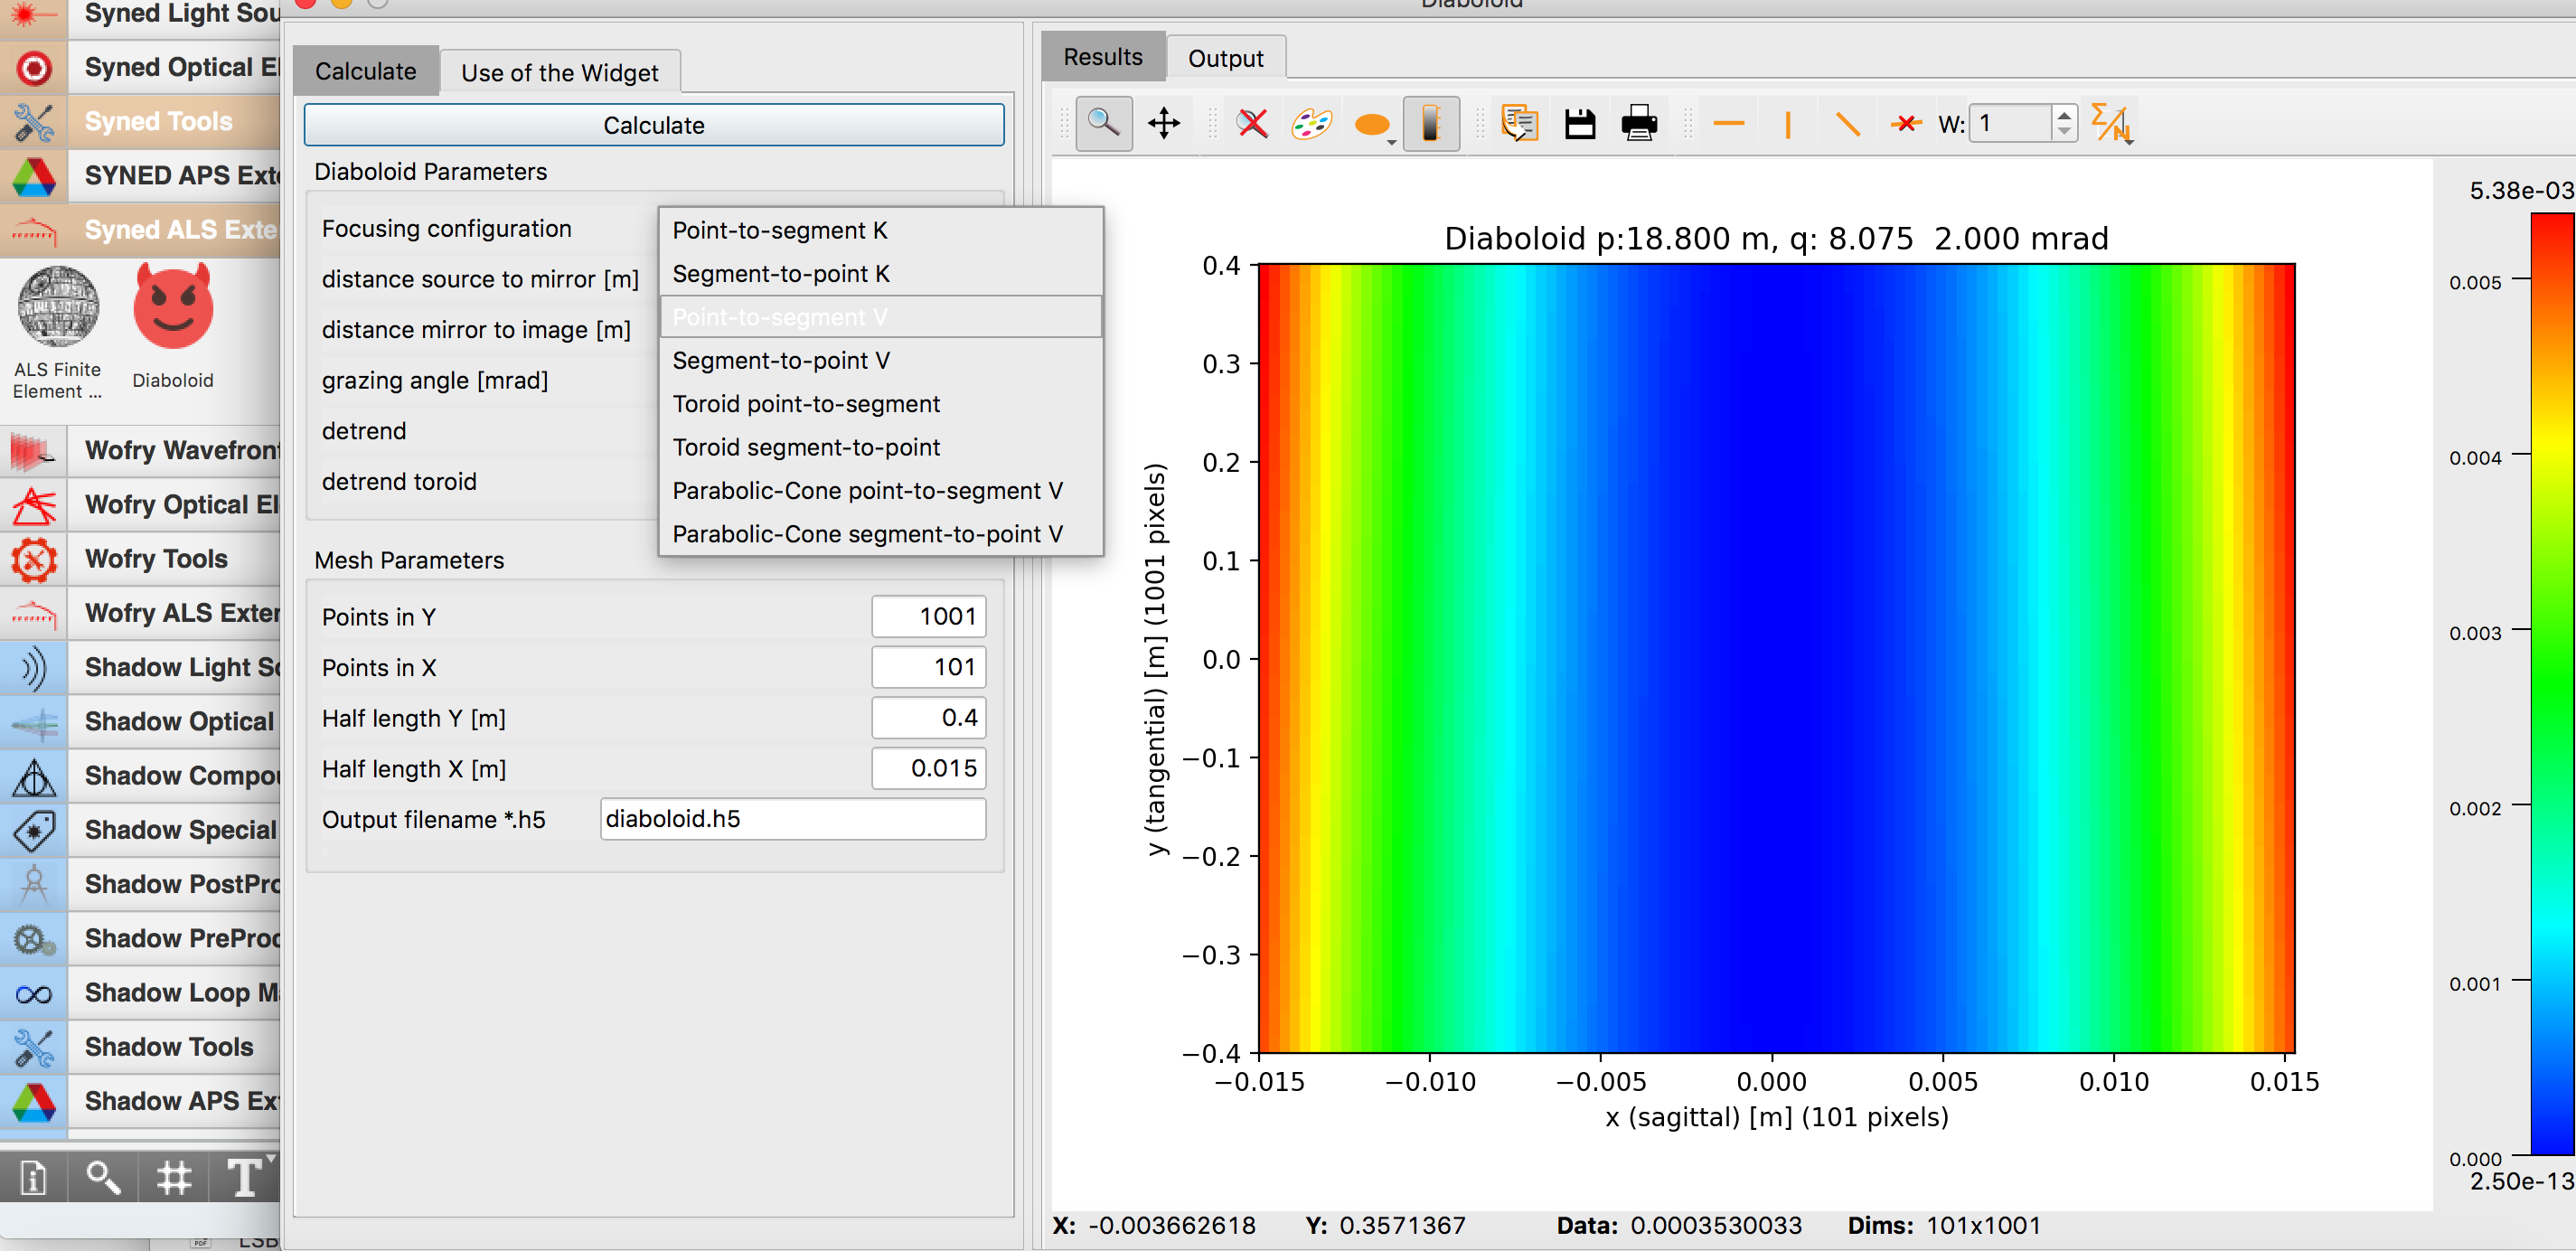
\includegraphics[width=0.95\textwidth]{figures/widget.png}
\caption{View of the interface to create the numerical sampling of the diaboloid and related surfaces (``Diaboloid" widget in Oasys/Syned).}
\end{figure}

To evaluate the accuracy of the calculations, we ray-traced an isolated diaboloid mirror. The simpler, point-to-segment, focusing configuration is chosen, with $p$~=~\SI{29.3}{\meter}, $q$~=~\SI{19.53}{\meter} and $\theta$~=~\SI{4.5}{\milli\radian}. A point source was modeled with divergence large enough to fully illuminate the mirror dimensions: length $L$~=~\SI{200}{\milli\meter}, and width $W$~=~\SI{20}{\milli\meter}.

\begin{figure}
\label{fig:pointToSegment}
\flushleft
~~~~a)~~~~~~~~~~~~~~~~~~~~~~~~~~~~~~~~~~~~~~~~~~~~~~b)\\
\centering
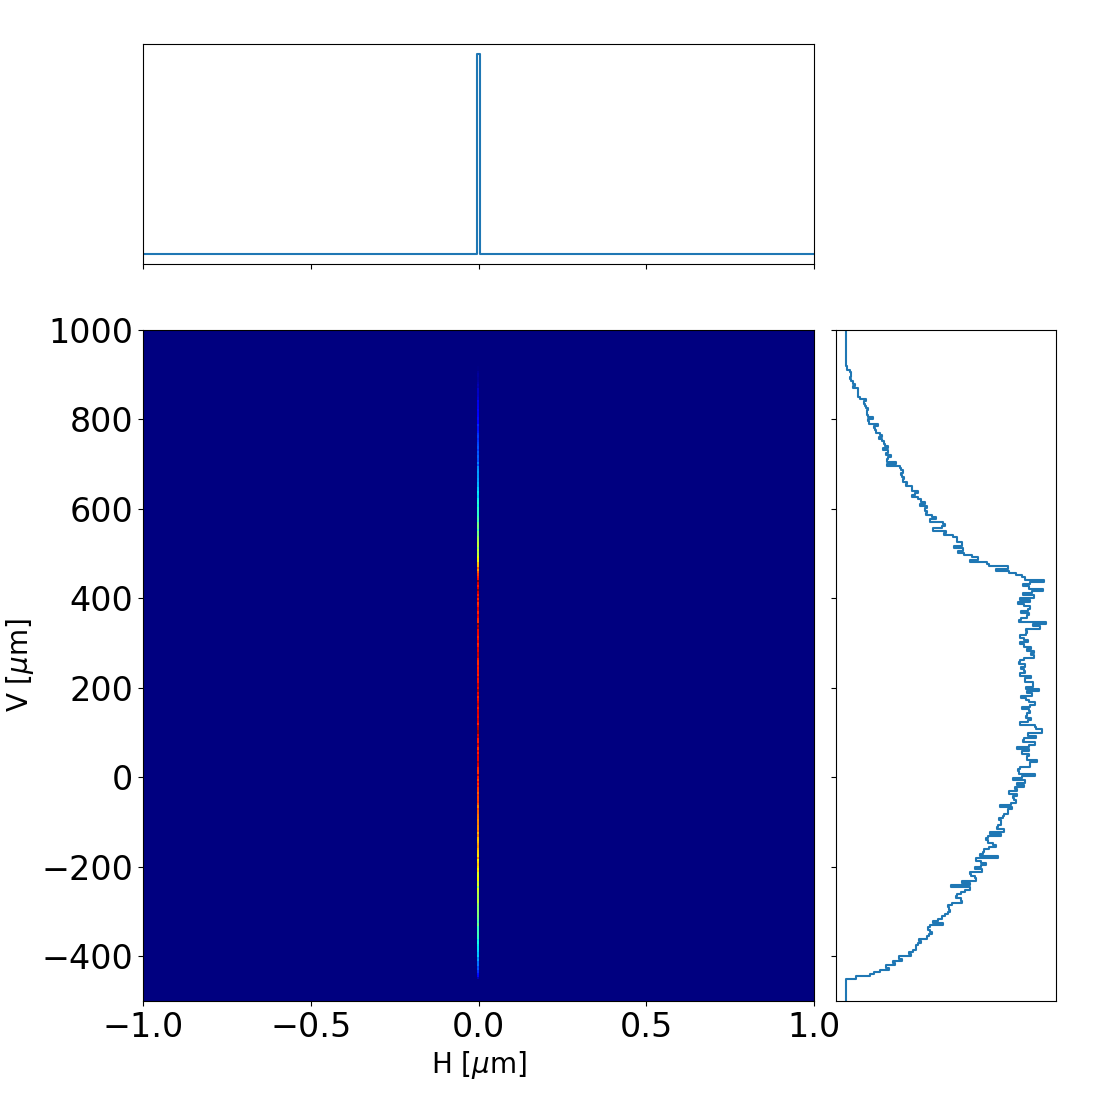
\includegraphics[width=0.49\textwidth]{figures/p2s_V_z.png}
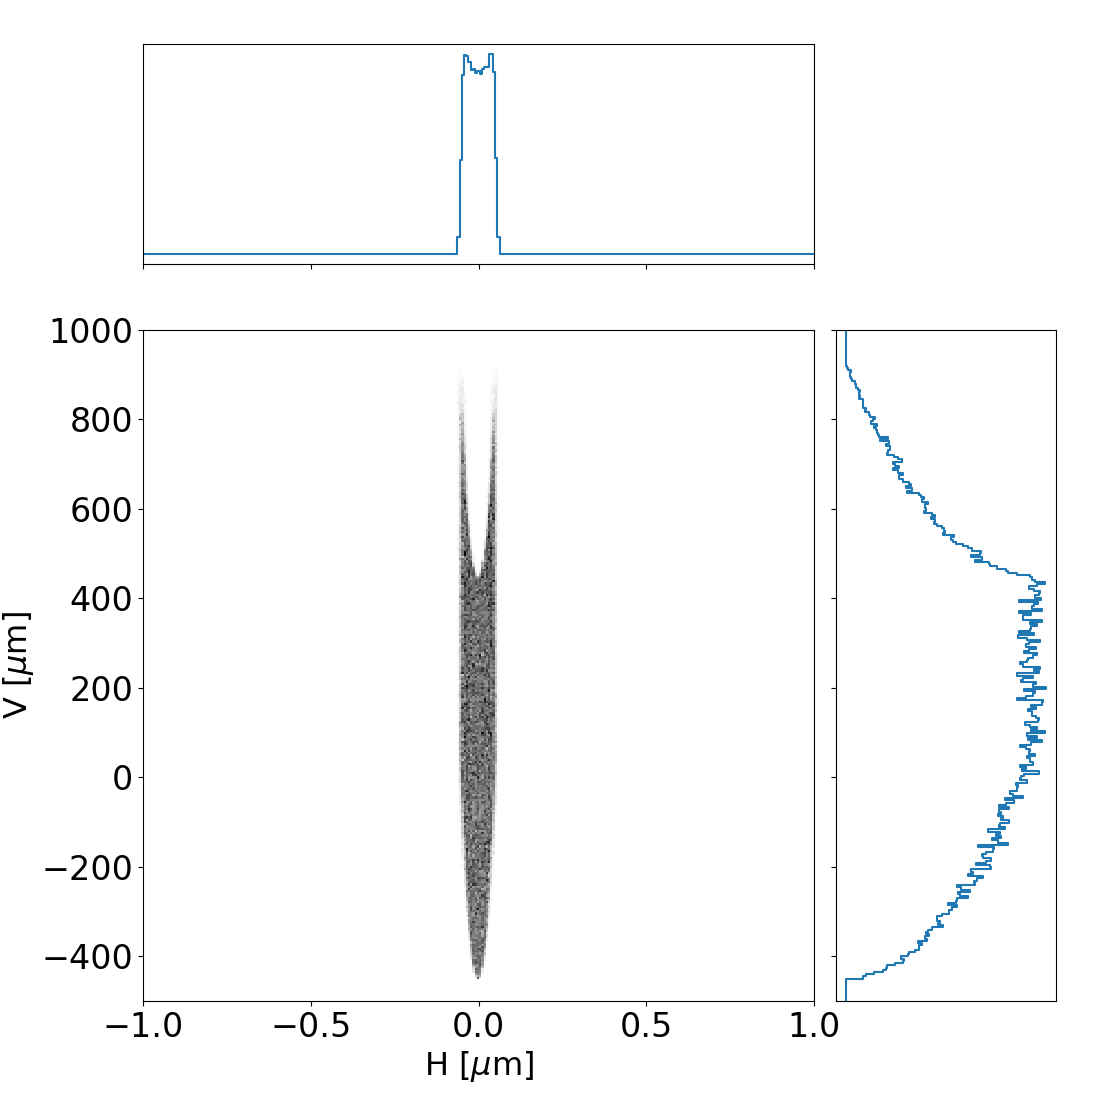
\includegraphics[width=0.49\textwidth]{figures/p2s_K_z.png} \\
\flushleft
\caption{Comparison of images produced by two surfaces: horizontally focusing and vertically collimating. (\textbf{a}) Exact diaboloid implementation (solving quartic equation), and (\textbf{b}) approximated implementation (equation~(\ref{eqn:diaboloidV}) detrended with $z_\mathrm{plane}=\theta Y$). The calculated FWHM values are \SI{0.3}{\nano\meter}, and \SI{93}{\nano\meter}, respectively.}
\end{figure}

The expected result at the focal position is a line focus (segment) \inblue{with zero horizontal width} \inred{(beam focused in horizontal)} \inblue{and a vertical length of $L\sin\theta$} \inred{(collimated in vertical, and considering full illumination of the mirror)}. Ray tracing focal images are shown in Fig.~\ref{fig:pointToSegment} for a diaboloid calculated with the two mentioned methods (exact solution and the detrended equation~(\ref{eqn:diaboloidV})). The intensity profile along the vertical direction has a non-uniform distribution due to the beam intensity projected on the mirror surface with a grazing angle.
\inred{This vertical intensity profile is invariant when the beam is propagated a long distance downstream from the image position, thus verifying the good collimation of the beam in the vertical plane.} Both numerical surfaces produce a narrow horizontal focus without aberration tails. However, some residual width is observed in the calculation: \SI{0.3}{\nano\meter} for the exact diaboloid equation and \SI{93}{\nano\meter} for the approximated one. The \SI{0.3}{\nano\meter} residual arises from the finite precision and from SHADOW's use of iterative algorithms to find ray intercepts.
The approximate diaboloid's \SI{93}{\nano\meter} residual comes from the linear detrending of the basal plane, replacing an exact rotation. We believe that this accuracy is sufficient for all current, practical implementations, owing to the finite source sizes of \SI{10}{\micro\meter} to \SI{50}{\micro\meter}. The approximate solution gives us an intuitive and simple direct way to numerically evaluate and visualize the surface.

\section{Ray tracing the ALS beamline 12.2.2}
\label{sec:beamline}

We analyze here the potential use of a diaboloid mirror to replace the toroid and upgrade the optical design of ALS Beamline 12.2.2 \cite{bl1222,MacDowell2004}. The beamline and its bending magnet source are evaluated at $E$~=~\SI{30}{\kilo\electronvolt} photon energy. We consider three source cases: i)~a point source; ii)~the ALS ring
$\sigma_x$~=~\SI{26}{\micro\meter}, $\sigma_y$~=~\SI{10}{\micro\meter}, 
electron energy $E_e$~=~\SI{1.9}{\giga\electronvolt}, magnetic field $B$~=~\SI{5.28}{\tesla}; and iii) the ALS-U ring, with $\sigma_x$~=~\SI{10}{\micro\meter}, $\sigma_y$~=~\SI{7}{\micro\meter}, $E_e$~=~\SI{2.0}{\giga\electronvolt}, and $B$~=~\SI{3.1}{\tesla}. 

Currently, the beamline uses a plane-parabola M1, and a toroidal M2. M1 vertically collimates the beam to optimize the monochromator performance (not simulated). M1 has $p_1$~= \SI{6.500}{\meter} from the source, and $q_1=\infty$, ($L$~= \SI{900}{\milli\meter} long, $\theta$~= \SI{2}{\milli\radian}). M2 focuses the vertically collimated, horizontally diverging beam to the exit slit. M2 has $p_2$~= \SI{18.800}{\meter} from the source and $q_2$~= \SI{8.075}{\meter}, ($L$~= \SI{800}{\milli\meter}, $W$~= \SI{20}{\milli\meter} wide, $\theta$~= \SI{2}{\milli\radian}). The exit slit (focal plane) is at $D$~= \SI{26.875}{\meter} from the source. The M2 magnification $M$ = $q_2/p_2$ = 0.43 is close but not exactly matching the optimal 1:2 toroid geometry \cite{MacDowell2004}.


\begin{figure}\label{fig:als}
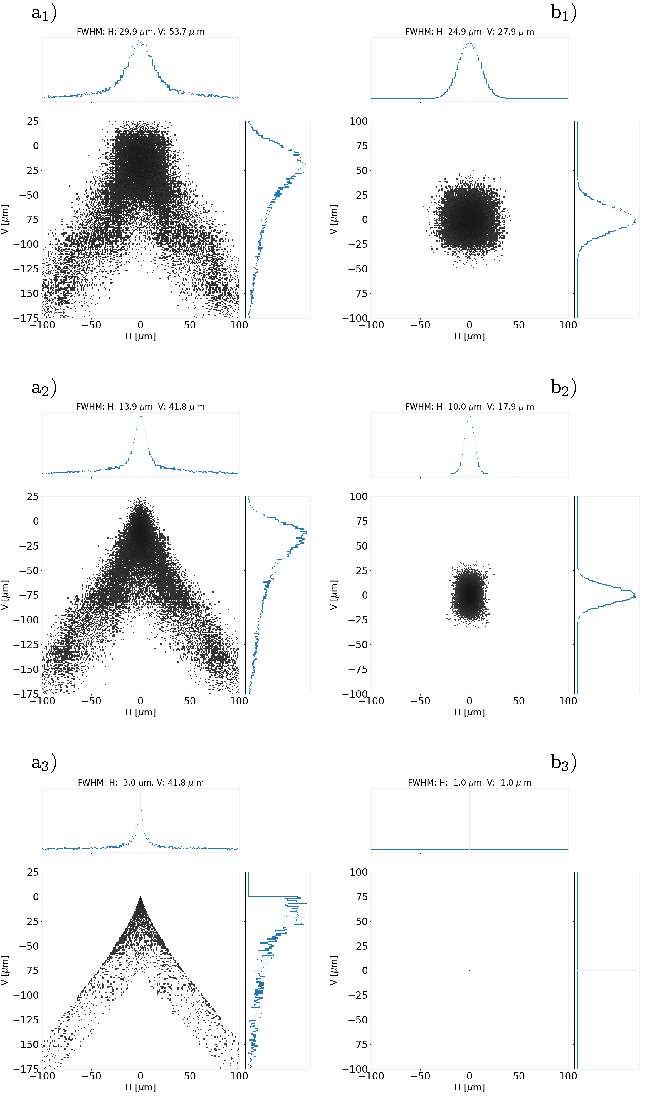
\includegraphics[width=0.85\textwidth]{figures/fig4.pdf}
\caption{Focal image produced by a system of two mirrors: M1 (collimating parabola) and M2 represented by (\textbf{a}) a toroid, or (\textbf{b}) a diaboloid. Row 1: bending magnet source in the current ALS storage ring. Row 2: the future, upgraded ALS-U ring. Row 3: ideal point source. The FWHM of the intensity distributions are written in the graphic titles. The image contrast is set to logarithmic scale for better visibility.}
\end{figure}

Figure~\ref{fig:als} compares the images produced by the three different sources and two mirror systems described above: toroid and diaboloid. With the current ALS case (Row 1), the diaboloid eliminates the tails but the reduction of the full width at half-maximum (FWHM) is only by a factor of 2 in the vertical direction, and less in the horizontal. Considering that the fabrication of diaboloid mirrors is still challenging, this mild improvement in focusing properties justifies the present use of toroids. However, for the ALS-U source (Row 2), focusing in the vertical direction gains a factor of 3 improvement in FWHM with the diaboloid, and eliminates the tails. In this case, we believe the diaboloid would provide a significant benefit. Row 3 shows the properties of these two optical systems with an ideal point source.

\section{The use of diaboloid for high demagnification}
\label{sec:scan}

Aberrations from the toroidal M2 increase as the magnification ratio changes away from the 1:2 condition. In an effort to achieve smaller spot sizes at the exit slit, we compare higher demagnification configurations. The existing toroid-containing design is extended for a reduction of the magnification ratio, $M=q/p$, and compared to an equivalent diaboloid design. We maintain a fixed M2 position ($p$), so the distance to the exit slit ($q$) and the length of the beamline must be reduced.

Figure~\ref{fig:demagnification} shows ray tracing simulations with $M$ reduced (from 0.43) to two specific values, 0.20 (1:5) and 0.10 (1:10). Relative to the small, Gaussian spots produced by the diaboloid, aberrations from the toroidal mirrors render these configurations unworkable.

\begin{figure}\label{fig:demagnification}
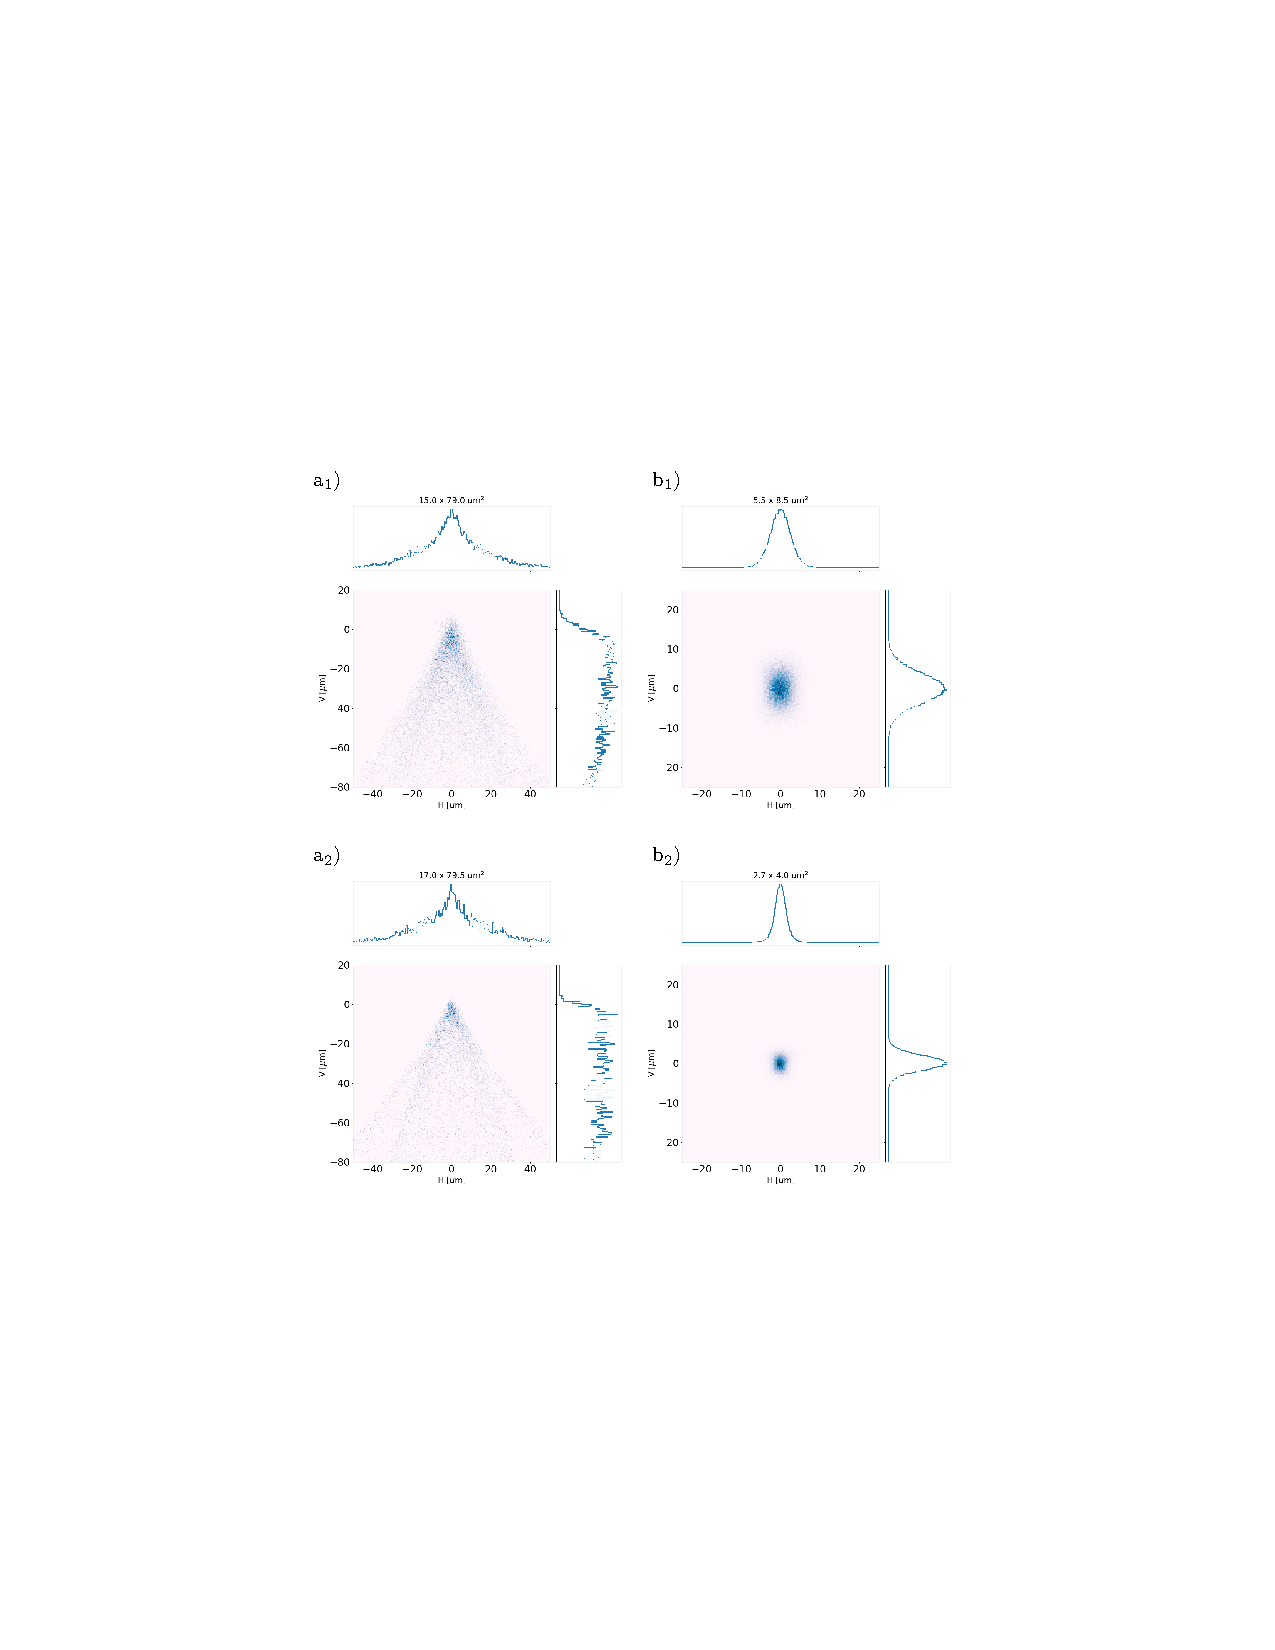
\includegraphics[width=1.0\textwidth]{figures/fig5.pdf}
% \flushleft
% ~~~~~a$_1$)~~~~~~~~~~~~~~~~~~~~~~~~~~~~~~~~~~~~~~~~~~~~~b$_1$) \\
% \centering
% 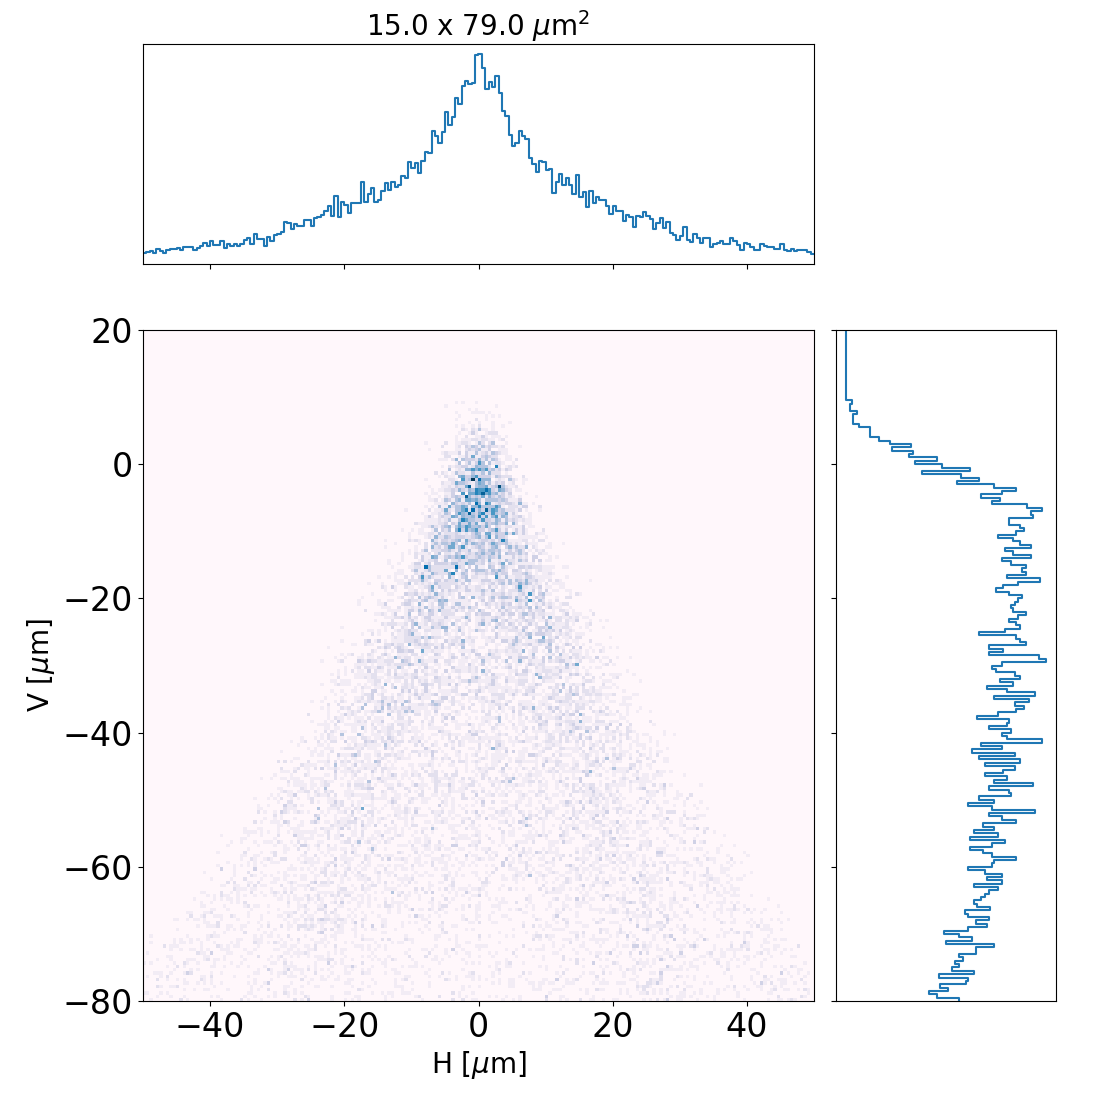
\includegraphics[width=0.45\textwidth]{figures/M0p2_toroid.png}
% 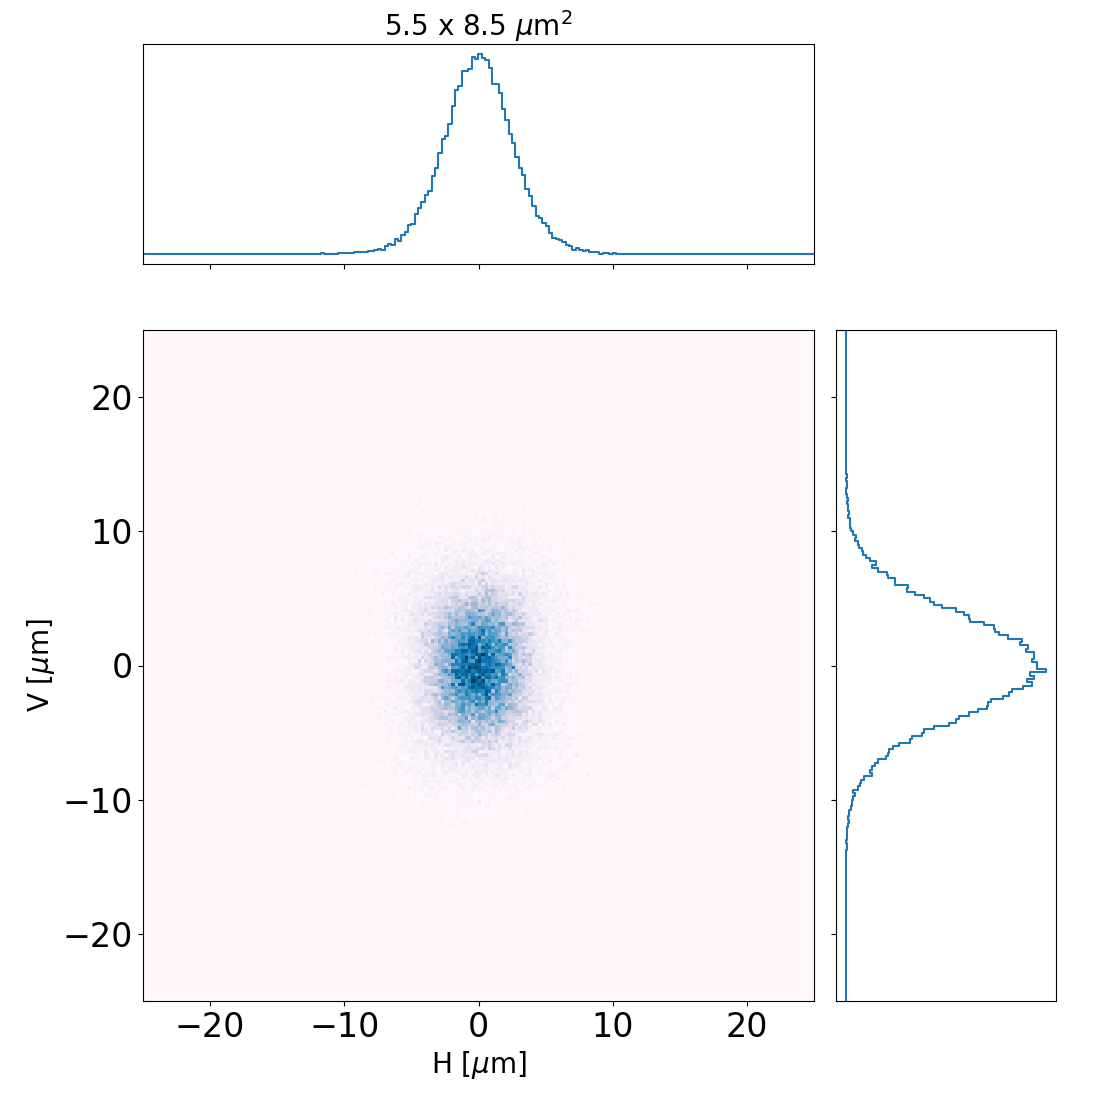
\includegraphics[width=0.45\textwidth]{figures/M0p2_diaboloid.png} \\
% 
% \flushleft
% ~~~~~a$_2$)~~~~~~~~~~~~~~~~~~~~~~~~~~~~~~~~~~~~~~~~~~~~~b$_2$) \\
% \centering
% 
% 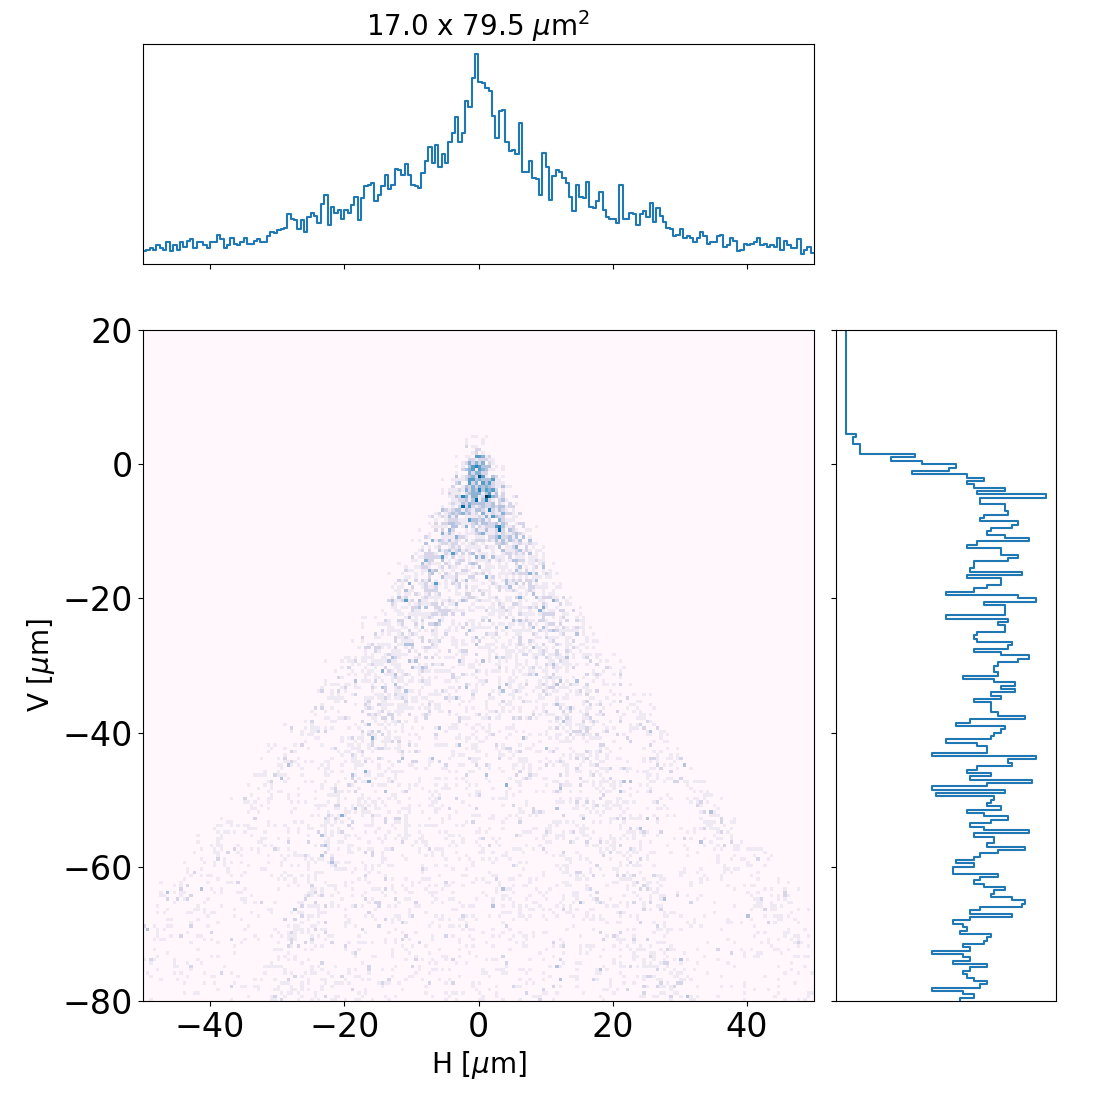
\includegraphics[width=0.45\textwidth]{figures/M0p1_toroid.png}
% 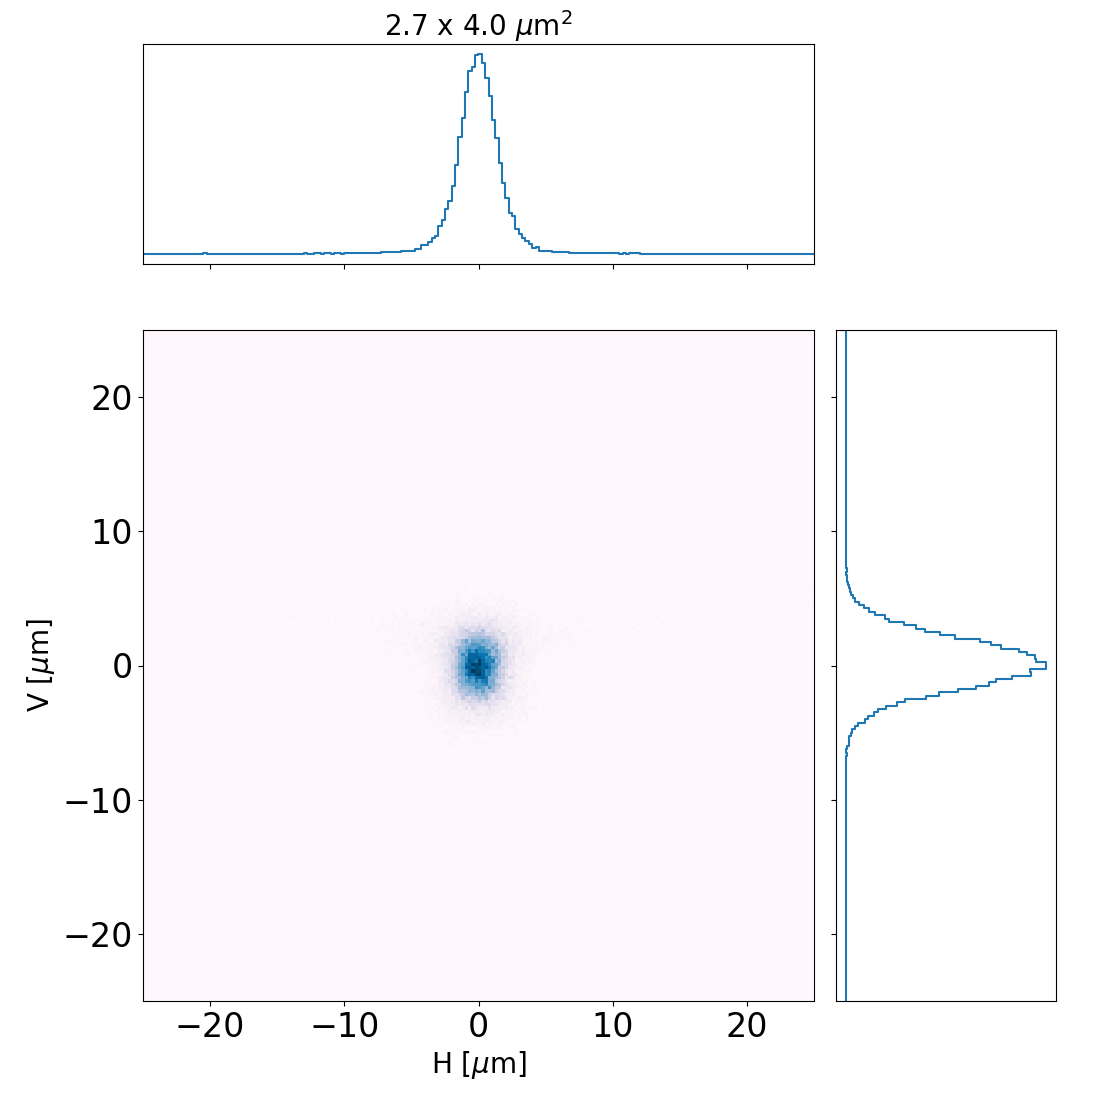
\includegraphics[width=0.45\textwidth]{figures/M0p1_diaboloid.png}
\caption{Image produced by the beamline for two magnification values: 1:5 (Row 1, top) and 1:10 (Row 2, bottom) using for M2 (\textbf{a}) a toroid, and (\textbf{b}) a diaboloid.}
\end{figure}

To study the aberrations in more detail, ray tracing calculations were performed \inred{for the ALS-U source}, scanning the magnification factor and extracting the focal dimensions, \inred{calculating both the $\sigma$ (RMS) and} the FWHM of the intensity distribution. A Gaussian distribution would show a ratio of FWHM/$\sigma$ of 2.35. The presence of aberrations rapidly increases $\sigma$ relative to the FWHM. The calculations are shown in Fig.~\ref{fig:scan}.

\begin{figure}\label{fig:scan}
\flushleft
a)\\
\centering
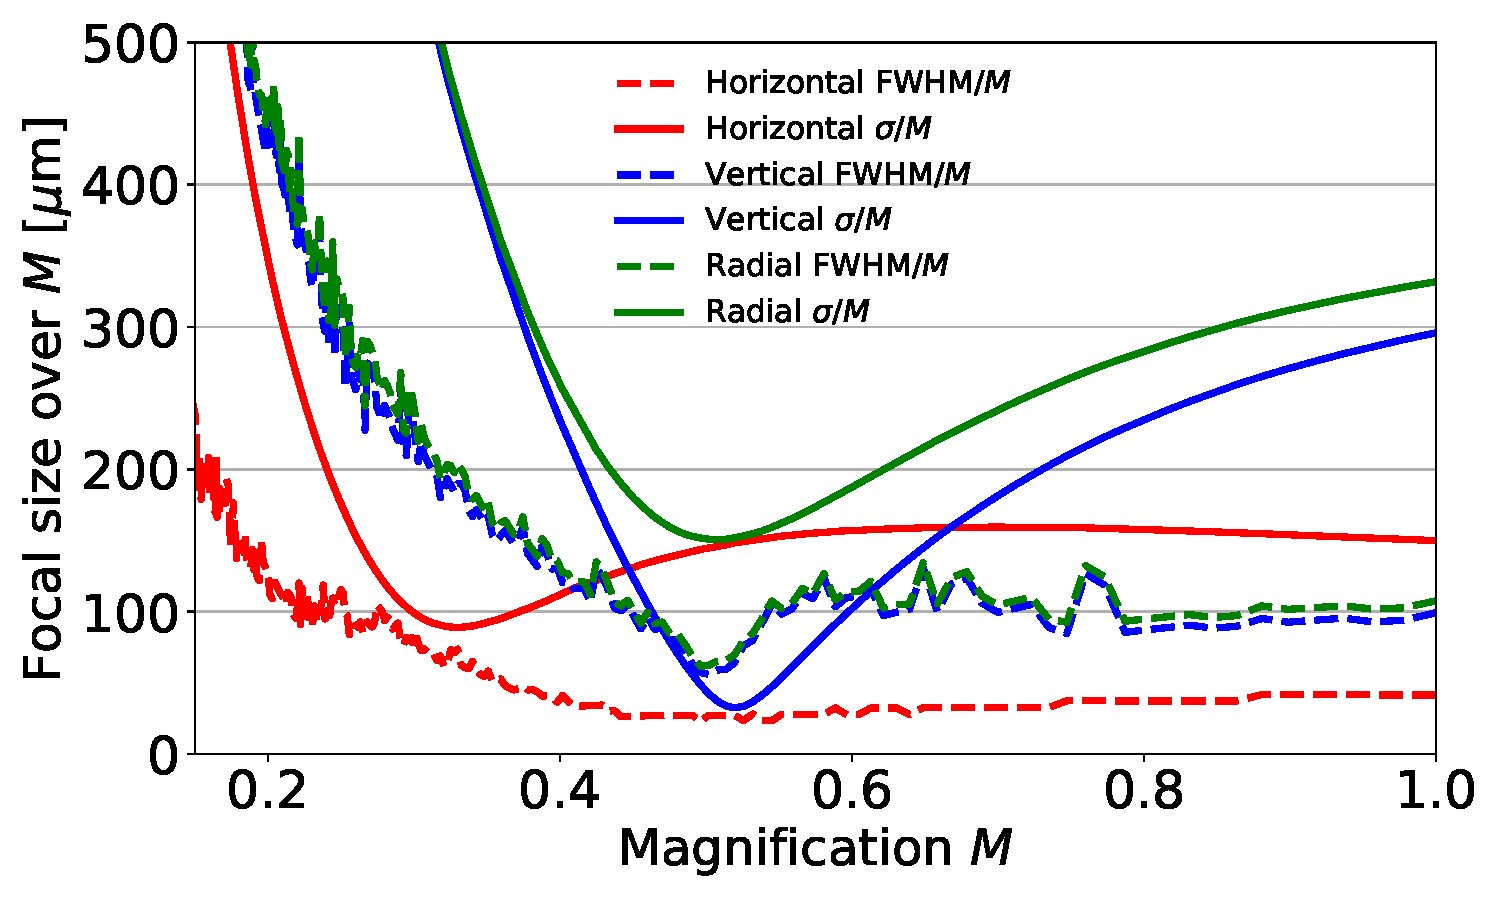
\includegraphics[width=0.95\textwidth]{figures/scan_toroid.pdf}\\
\flushleft
b)\\
\centering
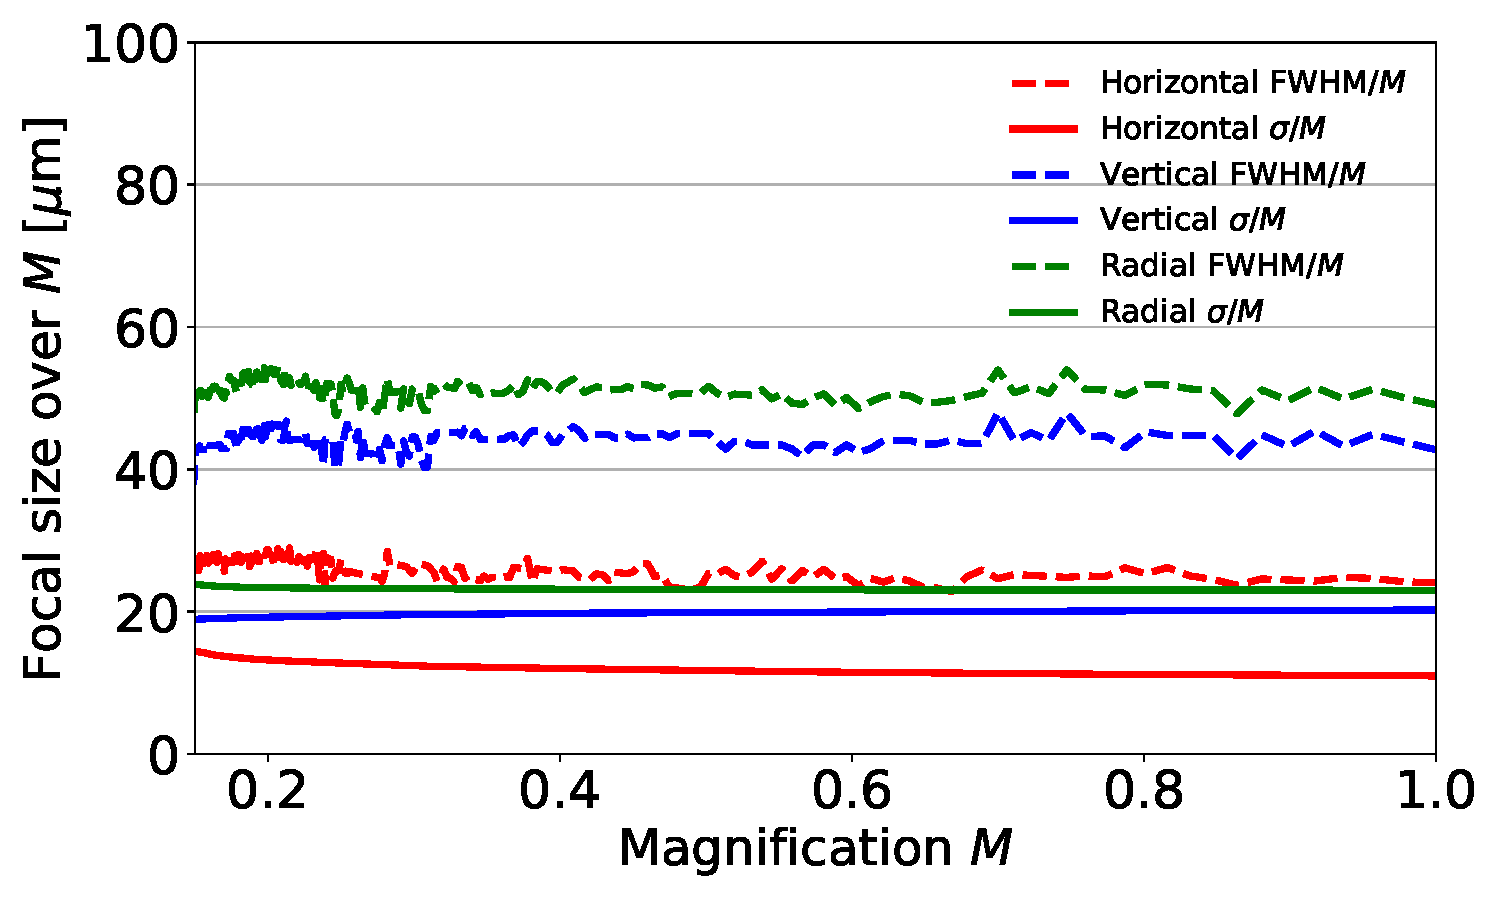
\includegraphics[width=0.95\textwidth]{figures/scan_diaboloid.pdf}\\
\caption{Calculated horizontal, vertical and radial focal sizes for a range of magnifications, measured by $\sigma$ and FWHM, and normalized to the magnification. We compare the (\textbf{a}) toroidal M2, and the (\textbf{b}) diaboloid. The normalized focal size should be constant for an ideal focusing system. \inred{The ALS-U source is considered.}}
\end{figure}

Normalizing the focal size to the magnification allows us to visualize the \inred{\sout{the}} broadening effects of the aberrations: the difference between the toroid and the diaboloid is apparent. Where $\sigma$ exceeds the fwhm, the aberrations are considered to be large. The toroidal mirror's radial aberrations $\sigma_r = (\sigma_h^2 + \sigma_v^2)^{1/2}$ (subindices $h$, $v$, and $r$ refer for horizontal, vertical and radial directions, respectively) are minimized for $M$~= 0.5, the 1:2 case, which is the ``working condition" for most ALS beamlines using toroids in this manner \cite{MacDowell2004}. For the diaboloid (Fig.~\ref{fig:scan}b), the situation is different: for most of the range ($M > 0.2$), the lines are almost constant and the $\sigma$ values are smaller than the fwhm by a ratio approaching 2.35. The diaboloids behave as ideal focusing optics.


\section{Study of mirror shapes that approximate the diaboloid}
\label{sec:approximatedShapes}

With its parabolic and elliptical cross sections, the diaboloid is a highly aspherical surface. Fabrication and metrology within the required accuracy levels are challenging technological problems. For this reason, we believe that the most favorable diaboloid shapes for manufacture are those that come closest to toroidal. With circular cross sections in both directions, toroids can be manufactured with high accuracy. To assess the manufacturing feasibility, we study the departure of the diaboloid from the toroidal surface with radii from equation~(\ref{eqn:radii}). The Oasys diaboloid was used to subtract a toroid from the diaboloid, point-by-point, for comparison.

In Fig.~\ref{fig:detrended} \inred{(top)} we have analysed diaboloid surfaces for three magnification ratios, $M$~= 0.2, 0.5, and 1.0 (1:5, 1:2 and 1:1), with \SI{2}{\milli\radian} grazing angle and a fixed \inred{horizontal} source distance, $p$~= \SI{20}{\meter}. In each case the toroid has been subtracted. Some sagittal profiles are also shown. 
\inred{The profiles at the center ($Y=0$) and at $Y=\pm$\SI{100}{\milli\meter} present a similar shape (an inverted ``U"), with a flat part at the middle ($|Y|<$\SI{5}{\milli\meter}).
% It can be appreciated in the magnification 1:5 ($p$~= \SI{20}{\meter}, $q$~= \SI{4}{\meter}) and 1:1 ($p$~= $q$~= \SI{20}{\meter}) a \inred{\sout{slight}} variation of the sagittal profile when going from
% However t
The change of height goes from about \SI{100}{\micro\meter} for $M=1:5$ to \SI{6}{\micro\meter} for $M=1:1$. 
}
At the 1:2 magnification condition, for a grazing angle of \SI{2}{\milli\radian} as used in ALS Beamline 12.2.2 (Fig.~\ref{fig:detrended}\inred{b}), the maximum difference from the toroidal shape is \SI{25}{\micro\meter}. For a grazing angle of \SI{5}{\milli\radian} as used in the protein crystallography beamlines (Fig.~\ref{fig:detrended}\inred{e}), the maximum difference is \SI{1.4}{\micro\meter} and the cross-sectional shape difference is almost uniform in the interval \inred{$|Y|<$\SI{200}{\milli\meter} along the} tangential direction.

\subsection{Considerations for diaboloid fabrication}
We observe that in the \SI{5}{\milli\radian} incidence case, the conversion of a cylindrical cross-section into an elliptical one, moving from the toroid to the diaboloid, could be done with a varied-thickness coating. The addition of a few microns of sputtered coating material
%\inred{coating material \sout{Si or Pt}}
on the Si substrate is practical and has been demonstrated \cite{Morawe}. In addition, at the 1:2 magnification condition, the mirror is close to a long elliptical cylinder. This should allow convenient ways to check the mirror height error using optical interferometry. Moreover, experience with long cylinders has shown that they can be produced with low tangential slope errors commensurate with the applications we envision. 

The deposition of a thin correcting layer
%at the edge of the 
\inred{on the} cylindrical substrate seems to be an attractive way to make diaboloids, at low glancing angles. % at least for the \SI{5}{\milli\radian} grazing angle case.
As sagittal slope errors are typically small, and the slope error tolerance in this direction is higher by $\sin\theta$, a method to create a diaboloid from a toroid is to first produce a sagittally varied coating on a flat substrate, or on a set of flat witness pieces along the length of the mirror. The variation in thickness could be created by a shaped mask in front of the sputtering source as the mirror is translated. Following this, the witness pieces will be examined by plane wave interferometry. This is now straightforward as the deviation from flat is small.
%, around 2 waves.
This allows calibration of the velocity of the mirror motion under the sputtering source, in order to get the right thickness at the edge of the aperture. Based on the highly repeatable deposition rates that can be produced with magnetron sputtering, we believe that we will be able to get the thickness at the edge within a few percent of the target, which is adequate in terms of an effective slope error. 

\begin{figure}\label{fig:detrended}
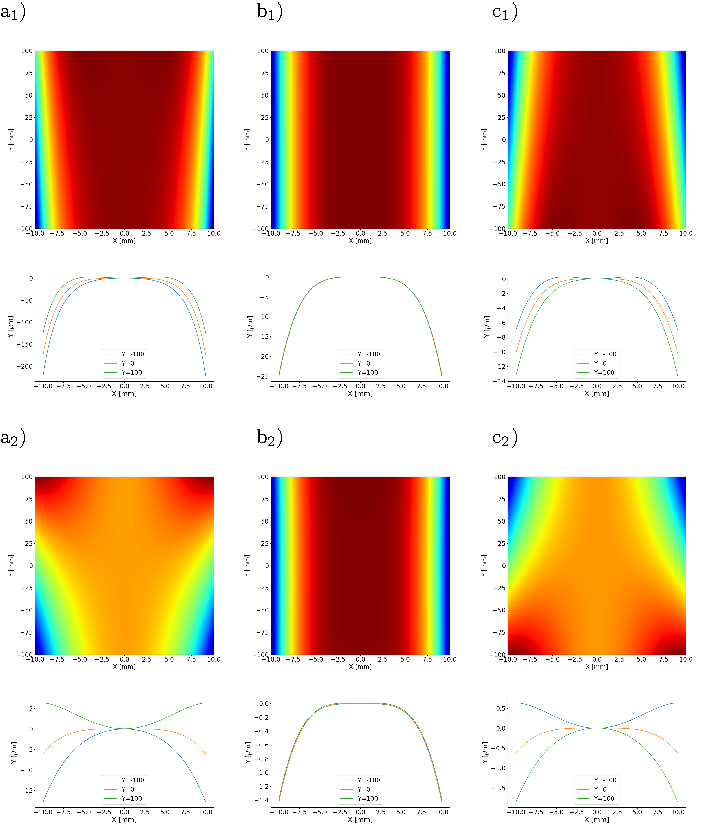
\includegraphics[width=1.0\textwidth]{figures/fig7.pdf}
% \flushleft
% a$_1$)~~~~~~~~~~~~~~~~~~~~~~~~~~~~~~~~~b$_1$)~~~~~~~~~~~~~~~~~~~~~~~~~~~~~~c$_1$)\\
% \centering
% 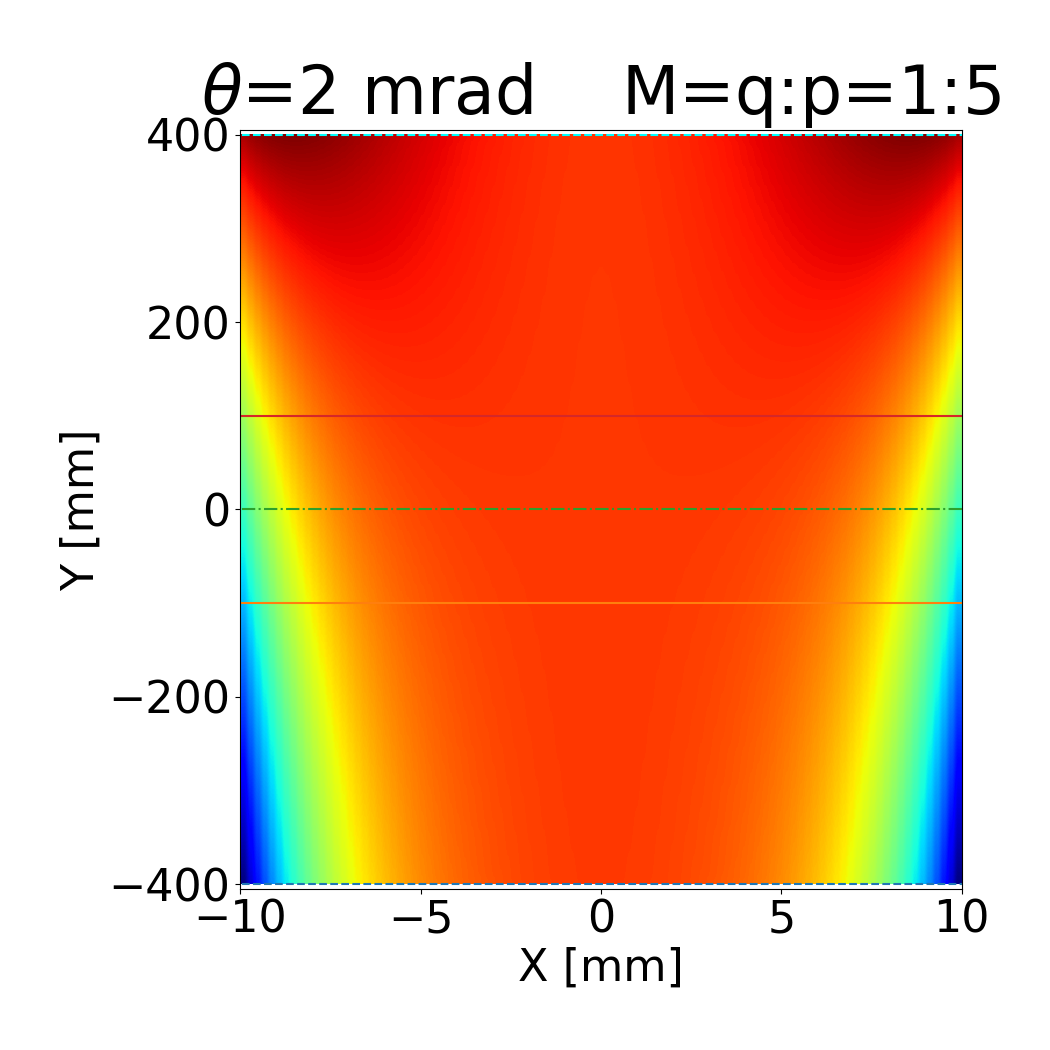
\includegraphics[width=0.32\textwidth]{figures/diaboloid_detrended_1:5_image.png} 
% 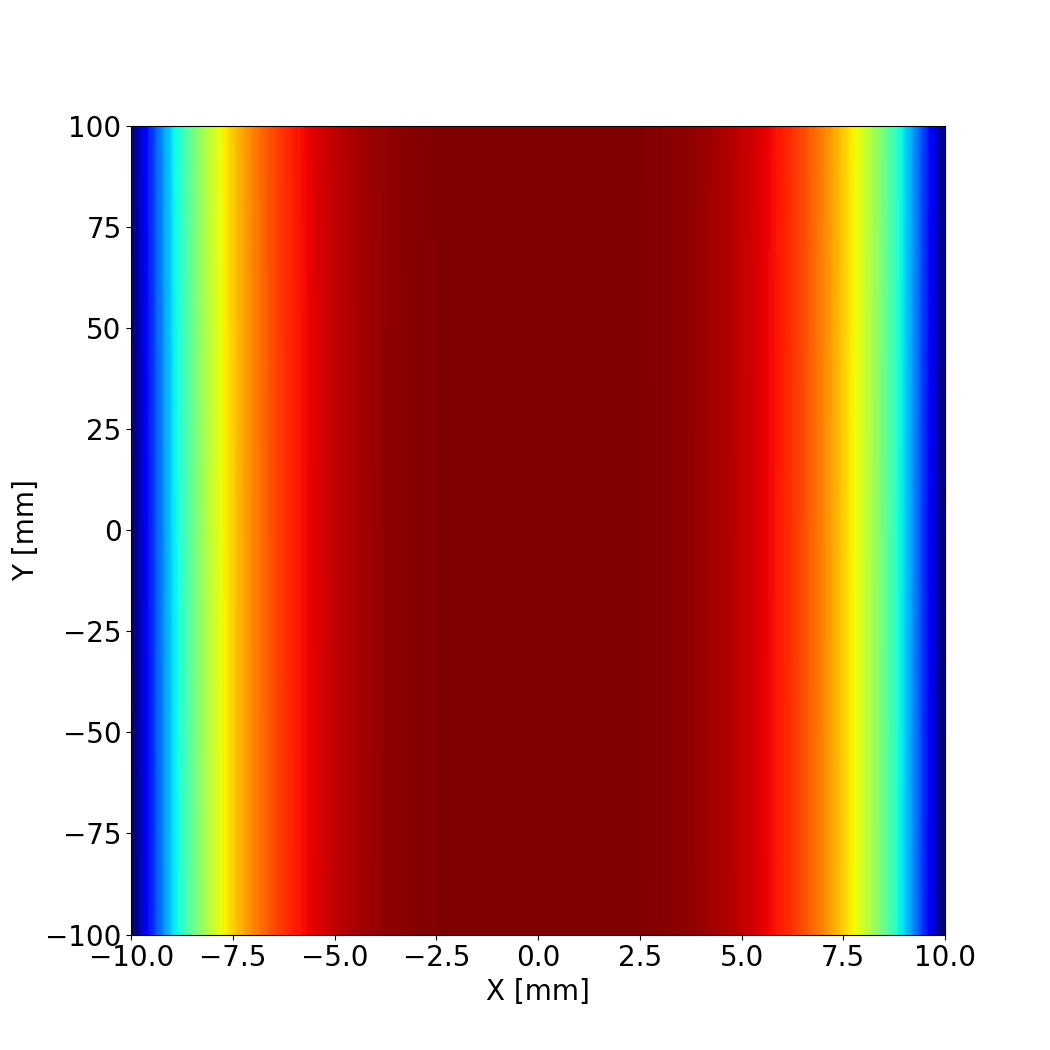
\includegraphics[width=0.32\textwidth]{figures/diaboloid_detrended_1:2_image.png} 
% 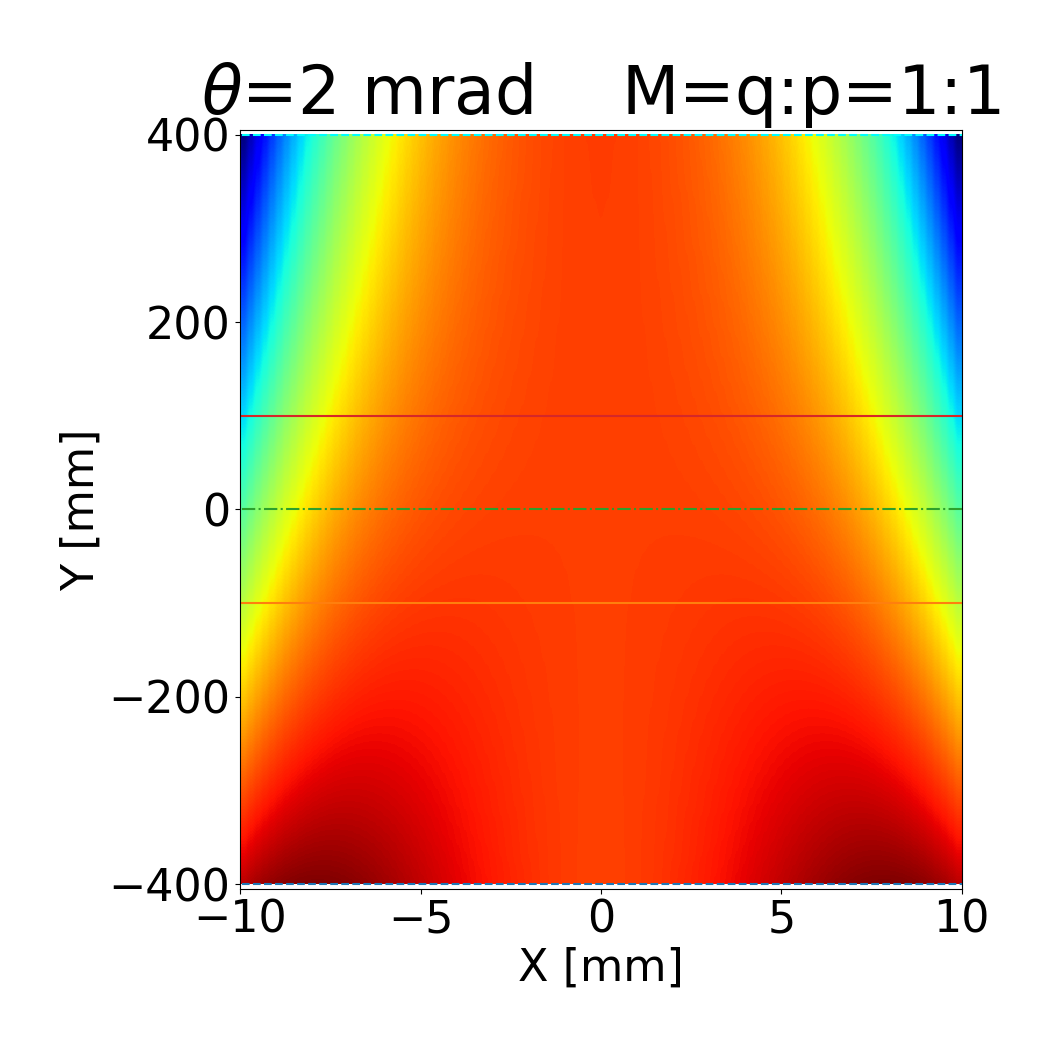
\includegraphics[width=0.32\textwidth]{figures/diaboloid_detrended_1:1_image.png} \\
% 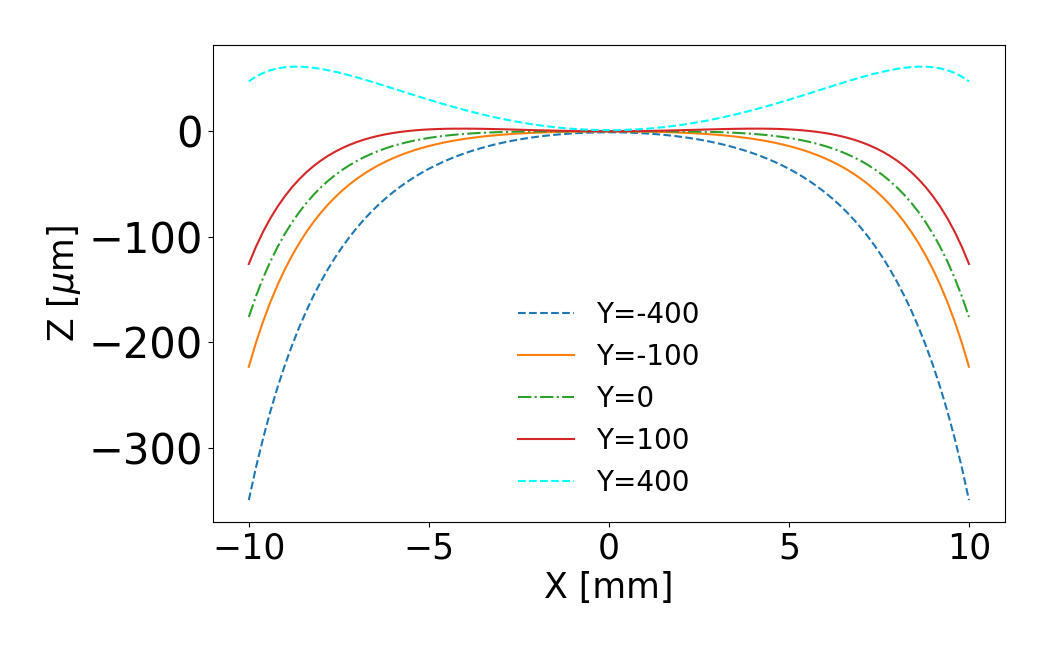
\includegraphics[width=0.32\textwidth]{figures/diaboloid_detrended_1:5_profile.png}
% 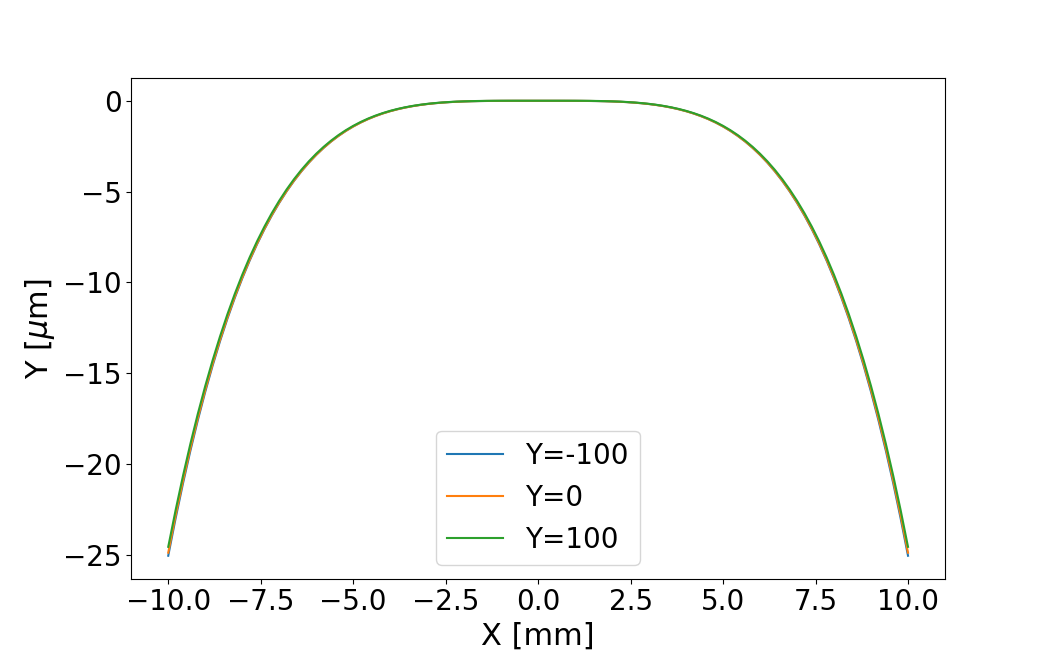
\includegraphics[width=0.32\textwidth]{figures/diaboloid_detrended_1:2_profile.png}
% 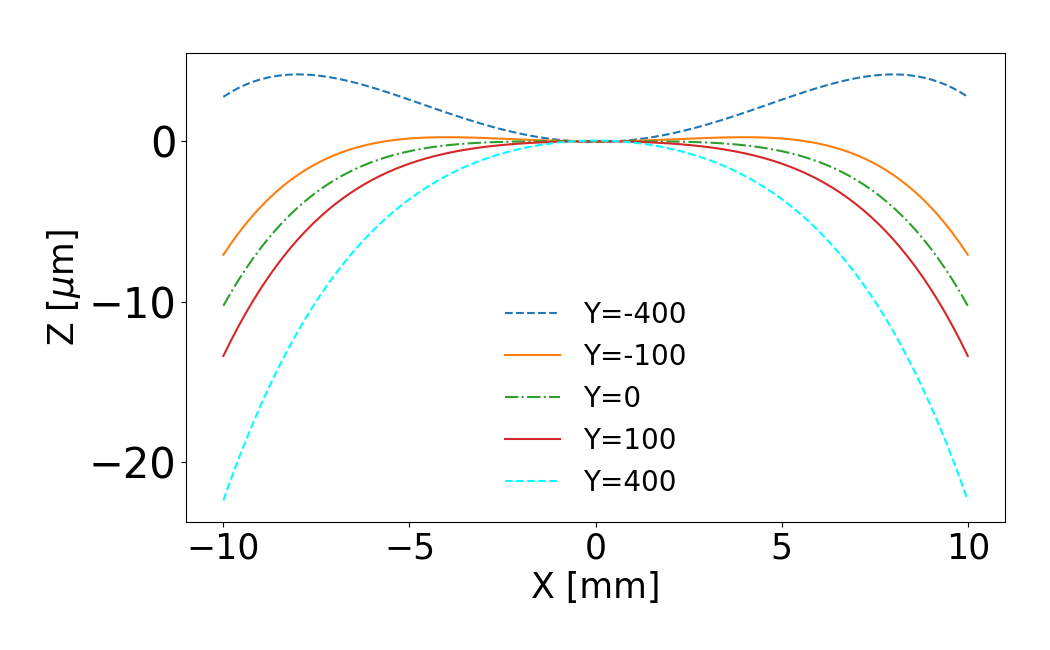
\includegraphics[width=0.32\textwidth]{figures/diaboloid_detrended_1:1_profile.png} \\
% \flushleft
% a$_2$)~~~~~~~~~~~~~~~~~~~~~~~~~~~~~~~~~b$_2$)~~~~~~~~~~~~~~~~~~~~~~~~~~~~~~c$_2$)\\
% \centering
% 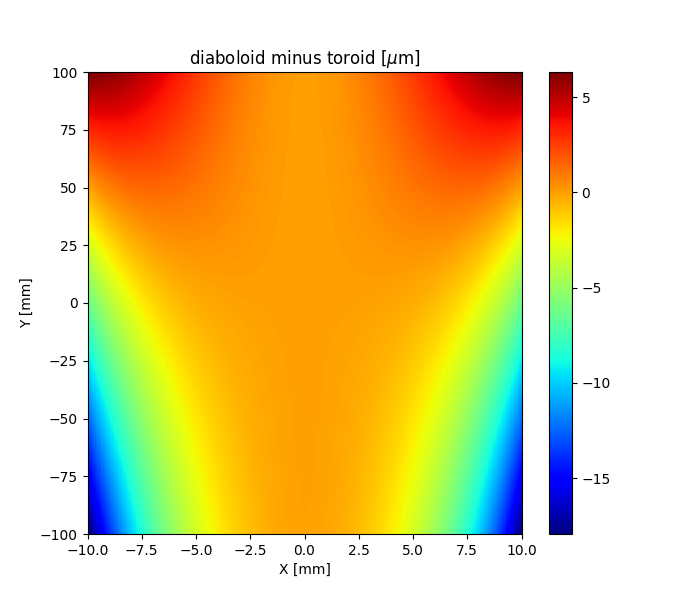
\includegraphics[width=0.32\textwidth]{figures/diaboloid_detrended_5mrad_1:5_image.png} 
% 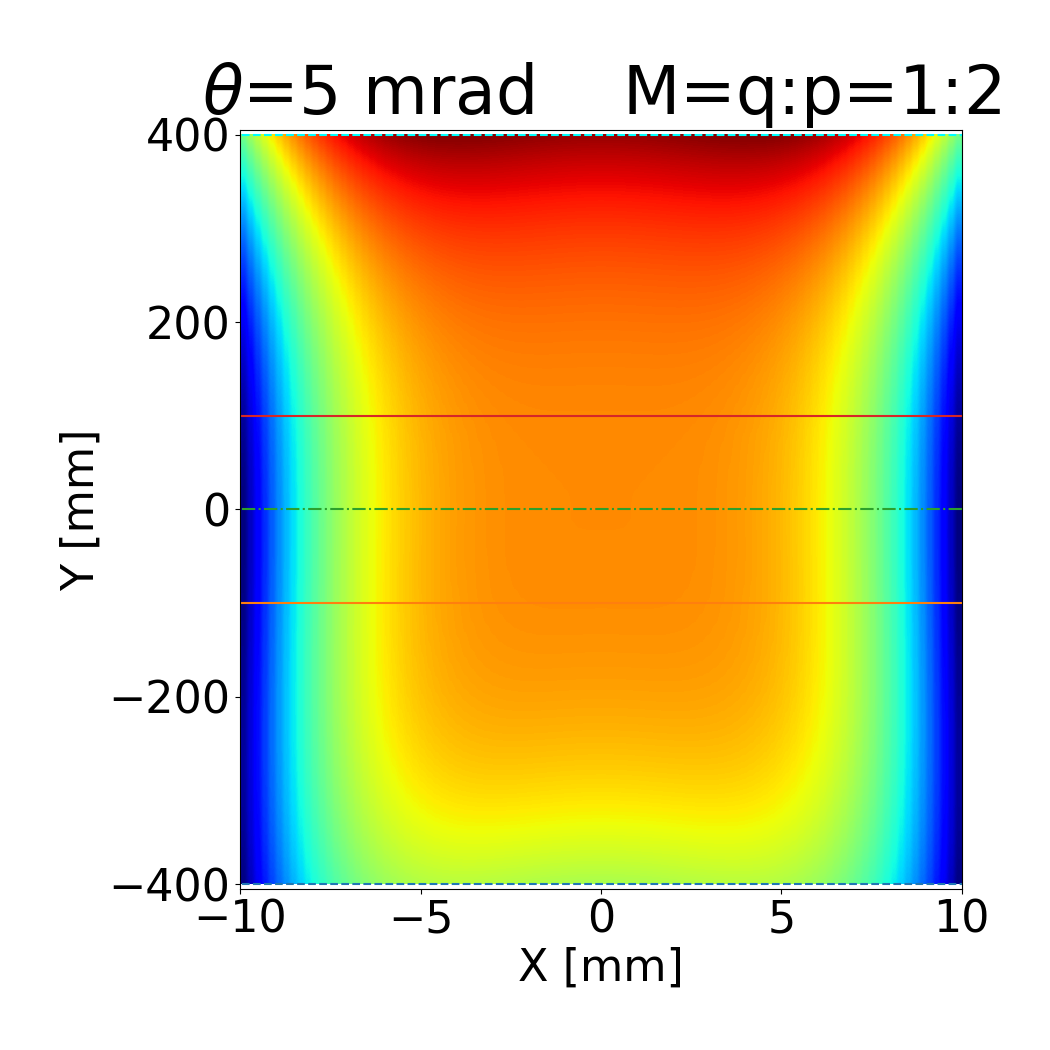
\includegraphics[width=0.32\textwidth]{figures/diaboloid_detrended_5mrad_1:2_image.png} 
% 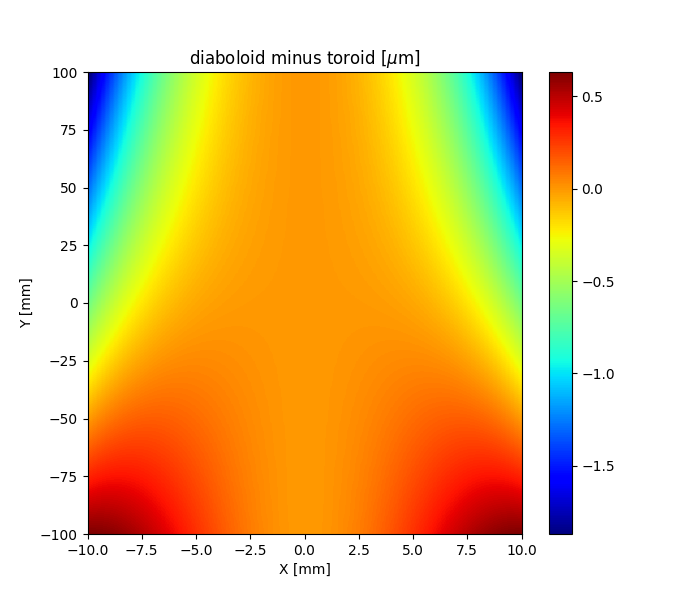
\includegraphics[width=0.32\textwidth]{figures/diaboloid_detrended_5mrad_1:1_image.png} \\
% 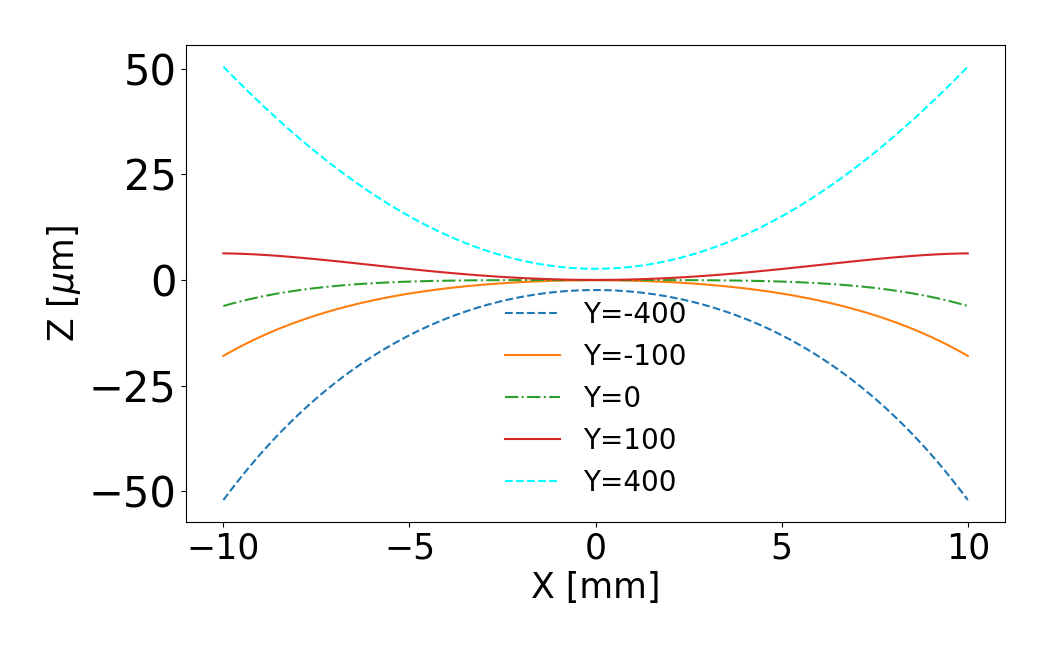
\includegraphics[width=0.32\textwidth]{figures/diaboloid_detrended_5mrad_1:5_profile.png}
% 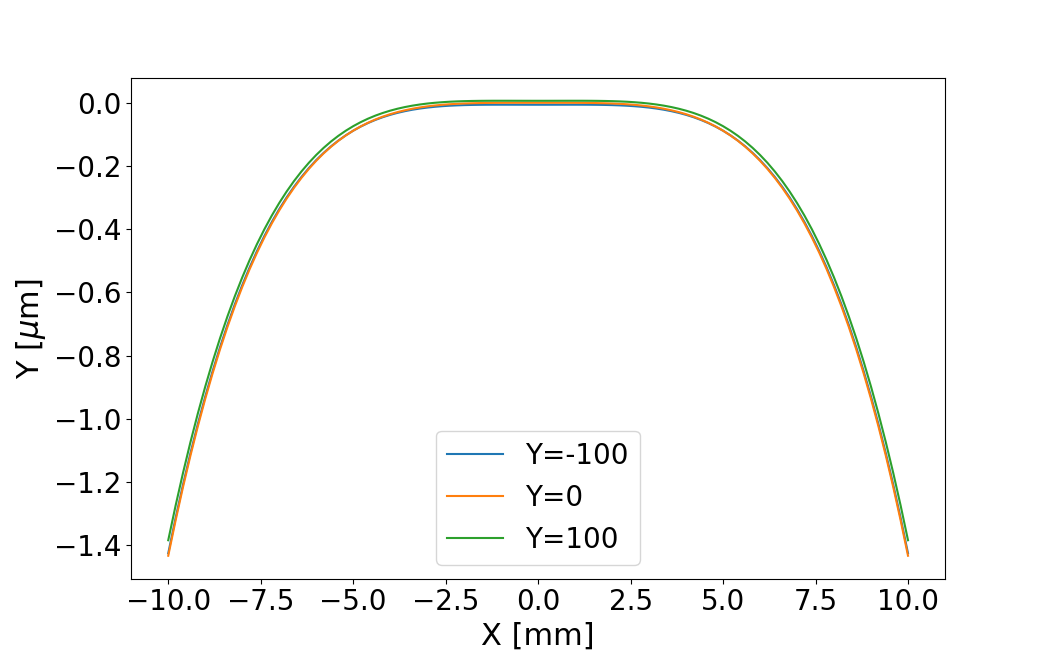
\includegraphics[width=0.32\textwidth]{figures/diaboloid_detrended_5mrad_1:2_profile.png}
% 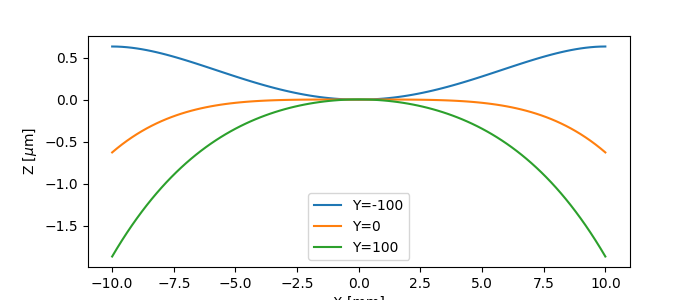
\includegraphics[width=0.32\textwidth]{figures/diaboloid_detrended_5mrad_1:1_profile.png}

\caption{Height difference between the diaboloid and the toroid for two different \inred{grazing angles (2 and \SI{5}{\milli\radian}) and three magnifications (1:5, 1:2 and 1:1). The values are shown at the image titles. For each image, five sagittal profiles at different $Y$ values are shown.} The simulations use a fixed \inred{horizontal} source distance, $p$~= \SI{20}{\meter}. In Row 1, the toroid major radii \inred{$R_t$} are \SI{4}{\kilo\meter}, \SI{10}{\kilo\meter}, and \SI{20}{\kilo\meter}, respectively; the minor radii \inred{$R_s$} are \SI{13.3}{\milli\meter}, \SI{26.7}{\milli\meter}, and \SI{40}{\milli\meter}. In Row 2, the toroid major radii are \SI{1.6}{\kilo\meter}, \SI{4.0}{\kilo\meter}, and \SI{8.0}{\kilo\meter}, respectively; the minor radii are \SI{33.3}{\milli\meter}, \SI{66.6}{\milli\meter}, and \SI{100}{\milli\meter}.}
\end{figure}

\subsection{Ray-tracing the approximate solutions}
We apply the manufacturing considerations to the case of the Beamline 12.2.2 after the ALS upgrade. The calculated focal spot size is 14 $\times$ \SI{42}{\micro\meter^2} (H $\times$ V) with a toroidal M2 mirror (Fig.~\ref{fig:als}a$_2$), and is 10 $\times$ \SI{18}{\micro\meter^2} with a diaboloid (Fig.~\ref{fig:als}b$_2$). As the situation is close to the 1:2 magnification and the incidence angle is \SI{2}{\milli\radian}, this is a promising case for upgrading the mirror to an approximated diaboloid. Fig.~\ref{fig:detrendedBeamline}a shows the difference between the diaboloid and the toroid. 

\begin{figure}\label{fig:detrendedBeamline}
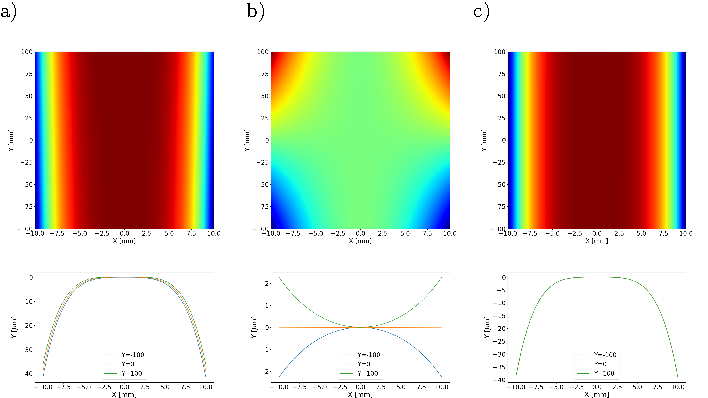
\includegraphics[width=1.0\textwidth]{figures/fig8.pdf}
% \flushleft
% a)~~~~~~~~~~~~~~~~~~~~~~~~~~~~~~~~~b)~~~~~~~~~~~~~~~~~~~~~~~~~~~~~~c)\\
% \centering
% 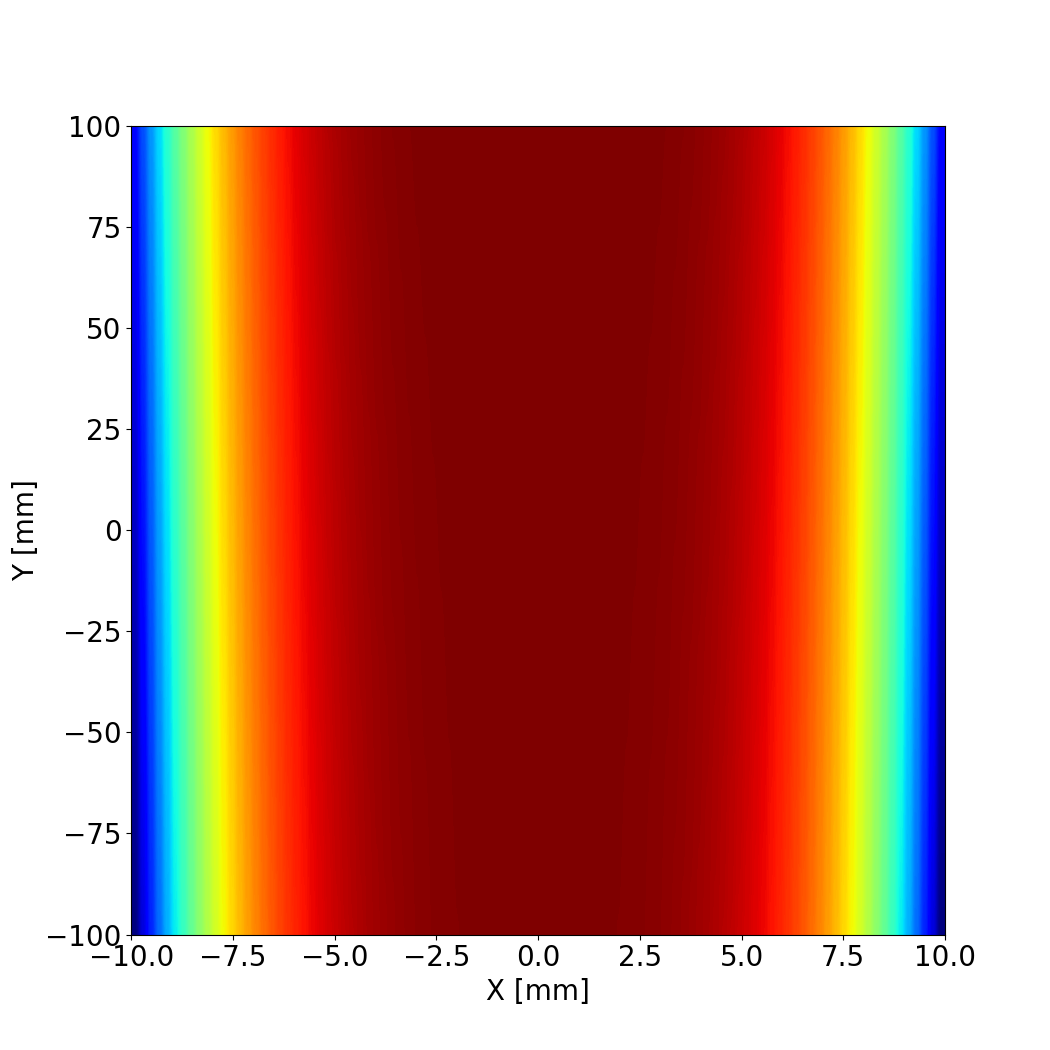
\includegraphics[width=0.32\textwidth]{figures/diaboloid_bl1222_detrended_image.png} 
% 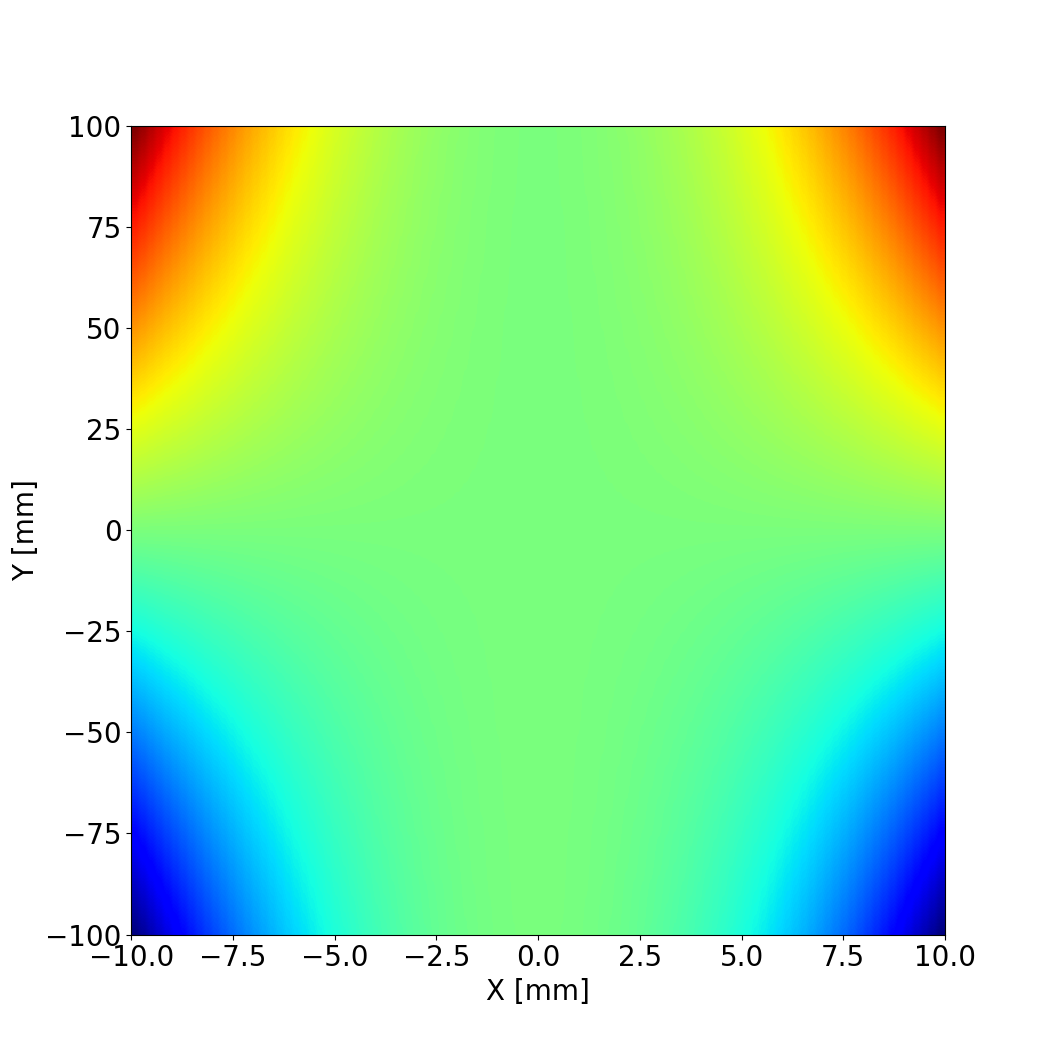
\includegraphics[width=0.32\textwidth]{figures/linearizedparaboliccone_bl1222_detrended_image.png} 
% 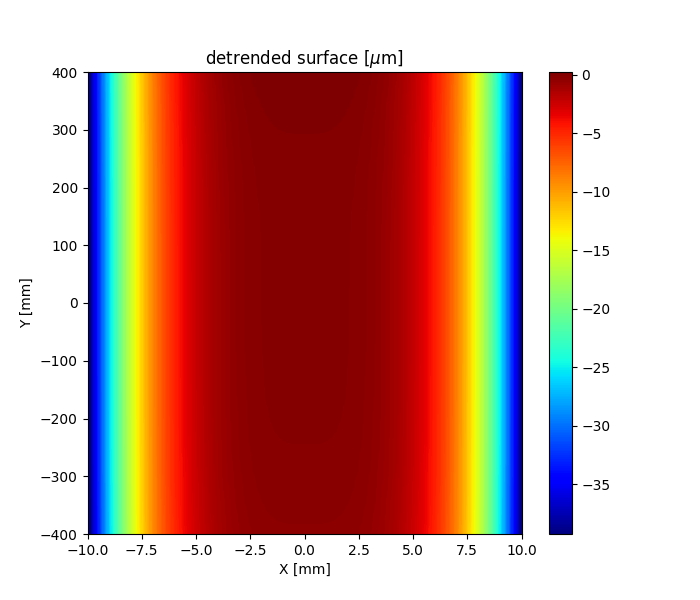
\includegraphics[width=0.32\textwidth]{figures/ellipticalcylinder_bl1222_detrended_image.png} 
% 
% 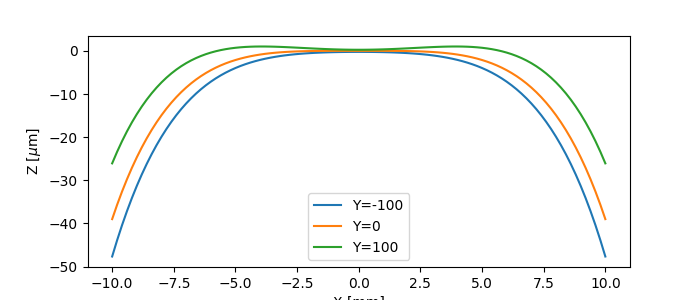
\includegraphics[width=0.32\textwidth]{figures/diaboloid_bl1222_detrended_profile.png}
% 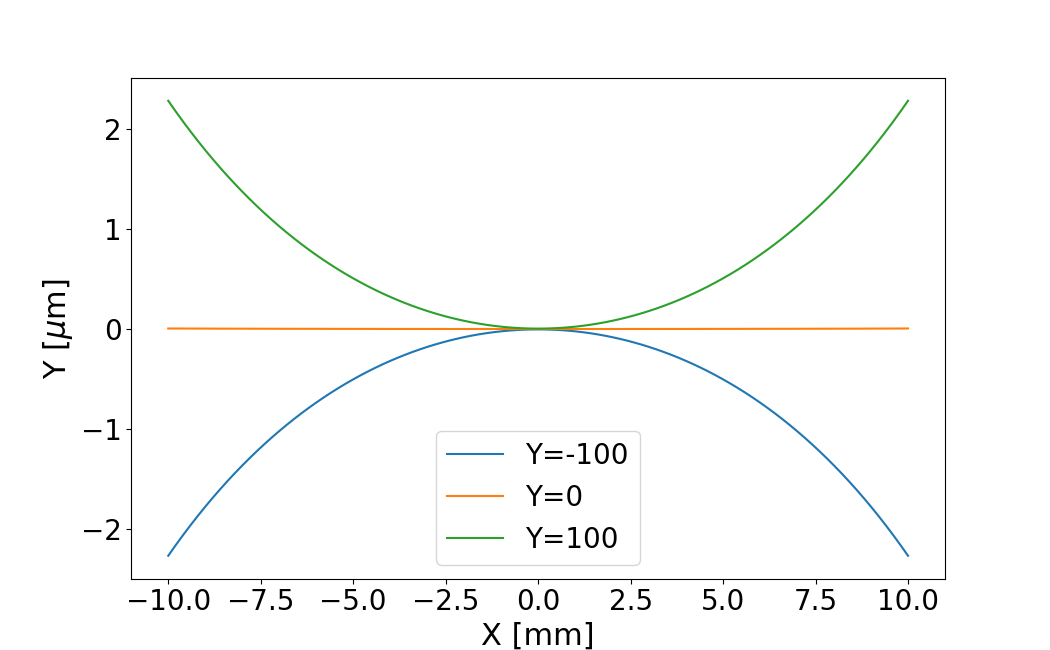
\includegraphics[width=0.32\textwidth]{figures/linearizedparaboliccone_bl1222_detrended_profile.png}
% 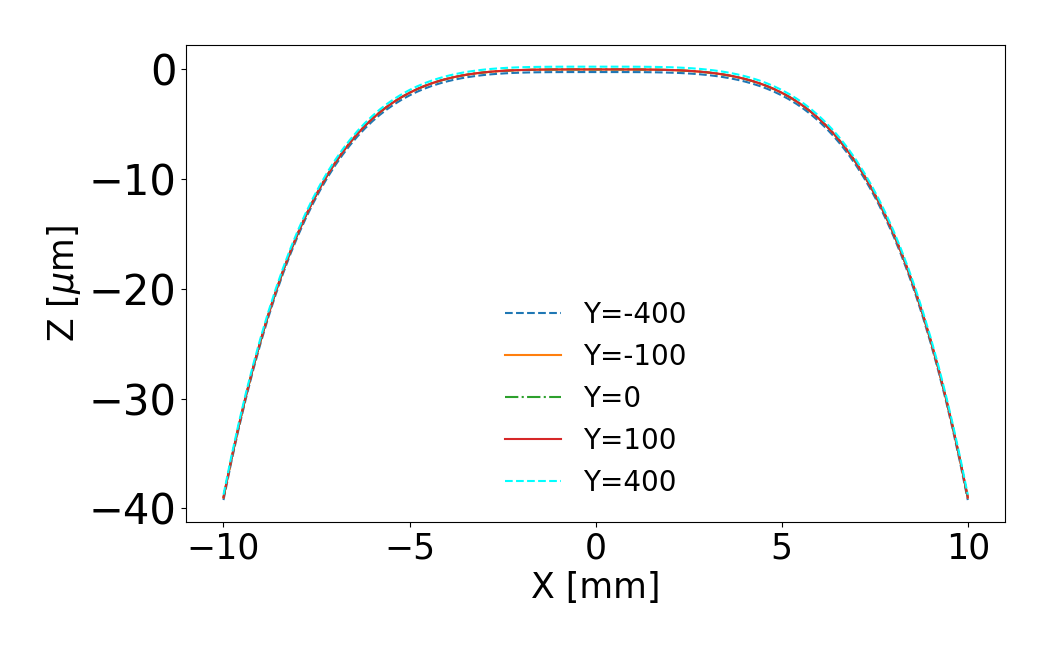
\includegraphics[width=0.32\textwidth]{figures/ellipticalcylinder_bl1222_detrended_profile.png}

\caption{Surface shapes for \inred{beamline} 12.2.2 with a toroid detrended and selected sagittal profiles: (\textbf{a}) diaboloid, (\textbf{b}) cone (equation~(\ref{eq:sagRadius})), and (\textbf{c}) elliptical cylinder bent to a parabola. The detrended toroid major radius is $R_t$~= \SI{8.075}{\kilo\meter} and the minor radius is $R_s$~= \SI{22.595}{\milli\meter}.}
\end{figure}

Two approximate solutions are studied by ray tracing. First, using a substrate with circular sagittal cross-sections, with a radius that changes linearly along the $Y$ (tangential) direction Fig.~\ref{fig:detrendedBeamline}b as indicated in equation~(\ref{eq:sagRadius}). The second one\inred{\sout{, more precise at a first view,}} would consist in pre-shaping a cylinder with elliptical sagittal cross-sections that matches the optimal sagittal profile at $Y$~= 0 (Fig.~\ref{fig:detrendedBeamline}c). Such a surface could be manufacturable with sufficient accuracy.

The spot size produced by the diaboloid is 10 $\times$ \SI{18}{\micro\meter^2} (Fig.~\ref{fig:als}b$_2$). The first approximation (cone bent to parabola) produces a spot of 12 $\times$ \SI{23}{\micro\meter^2} (Fig.~\ref{fig:finalcomparison}a). In the case that this cone is degenerated into a cylinder, the size becomes 14 $\times$ \SI{33}{\micro\meter^2} and an aberration tail appears in vertical direction (Fig.~\ref{fig:finalcomparison}b). This is due to this beamline being close but not exactly at 1:2 magnification (it is exactly M = 
% $q$:$p$ = 8.075:18.800
\inred{1:2.33}). If using the second approximation (cylinder with elliptical section) we obtain: 16 $\times$ \SI{38}{\micro\meter^2} with a strong aberration tail, for the same reason (Fig.~\ref{fig:finalcomparison}c).
In the horizontal direction, the mirror with sagittal elliptical cross-sections produce \inred{larger} focal spots (Fig.~\ref{fig:finalcomparison}c) than those with circular cross-sections (Fig.~\ref{fig:finalcomparison}a and b). \inred{This may result paradoxal at a first view, but shows a cross-over between tangential and sagittal directions: to improve the sagittal focus, it is preferred to use the circular section but with changing curvature along the tangential direction, rather than use the ideal sagittal profile (ellipse) without change along the tangential direction. }

We check now the beamline in a optimal 1:2 configuration, by setting $q$~= \SI{9.4}{\meter}. Here the diaboloid produces a spot of 12 $\times$ \SI{22}{\micro\meter^2} (not shown), 13 $\times$ \SI{26}{\micro\meter^2} for the cone and \inred{the same} for the circular cylinder (Fig.~\ref{fig:finalcomparison}d), as expected because for 1:2 magnification the cone degenerates in a cylinder. The result for the elliptical cylinder is similar (not shown), demonstrating that there is not much benefit in this case to shape the cylinder with a more complicated elliptical section.  

In conclusion, the approximation of the diaboloid by a simple circular cylinder bent to a parabola works well at exactly 1:2 magnification. However at even small deviations from the 1:2 condition, as in the present ALS Beamline 12.2.2 case, the approximation of the diaboloid by a cone has to be used to eliminate the asymmetric aberration tail in tangential direction. For other magnifications the exact diaboloid should be used.


\begin{figure}\label{fig:finalcomparison}
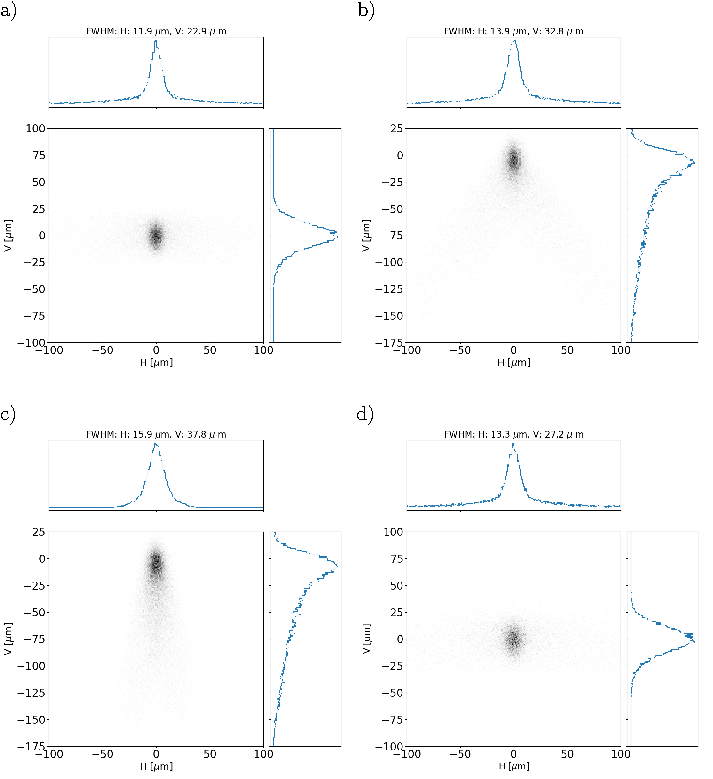
\includegraphics[width=1.0\textwidth]{figures/fig9.pdf}
% \flushleft
% a)~~~~~~~~~~~~~~~~~~~~~~~~~~~~~~~~~~~~~~~~~~~~~~~~~b)\\
% \centering
% 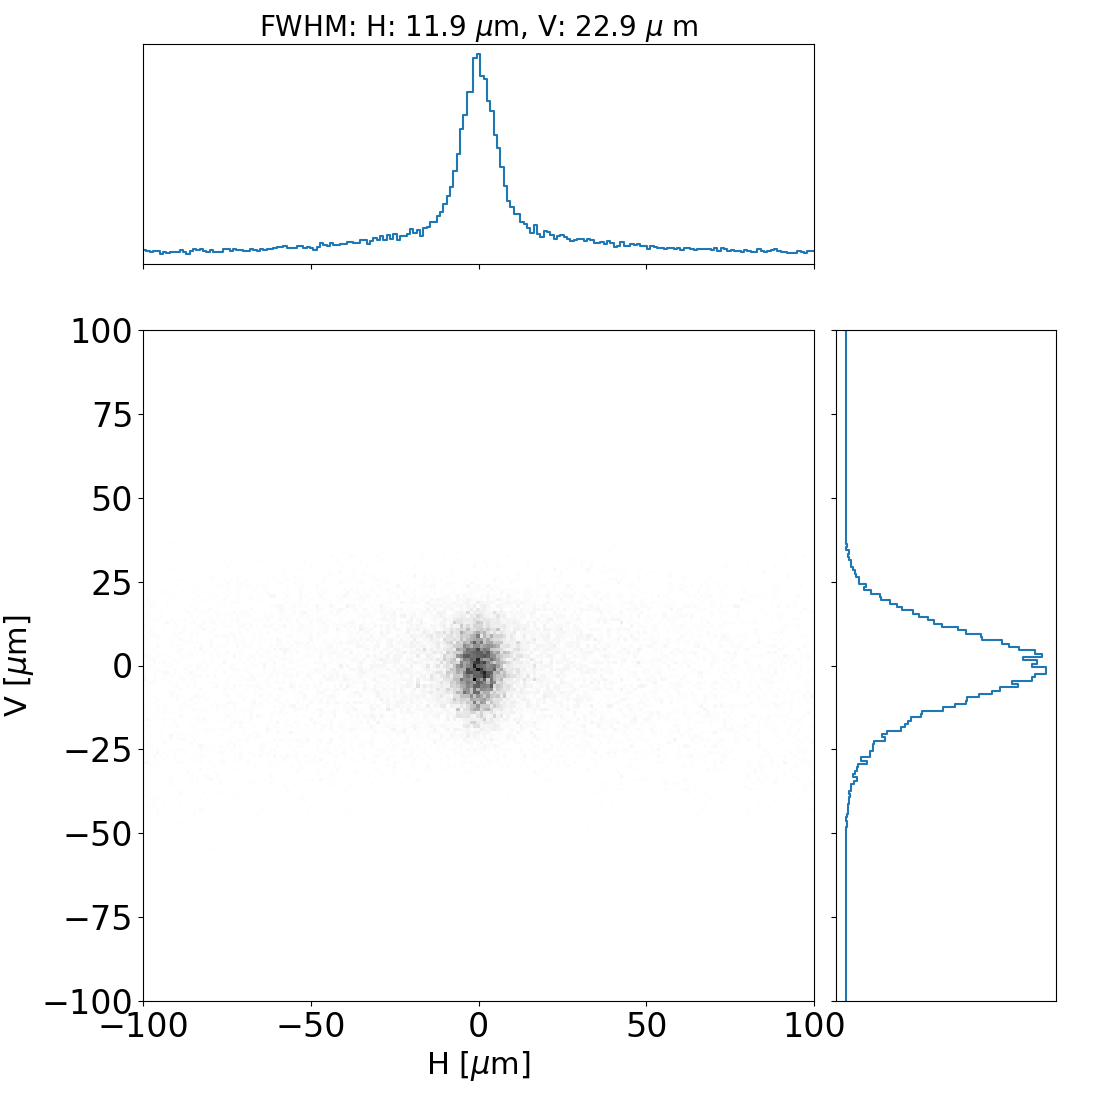
\includegraphics[width=0.49\textwidth]{figures/prefinal_approx1.png} 
% 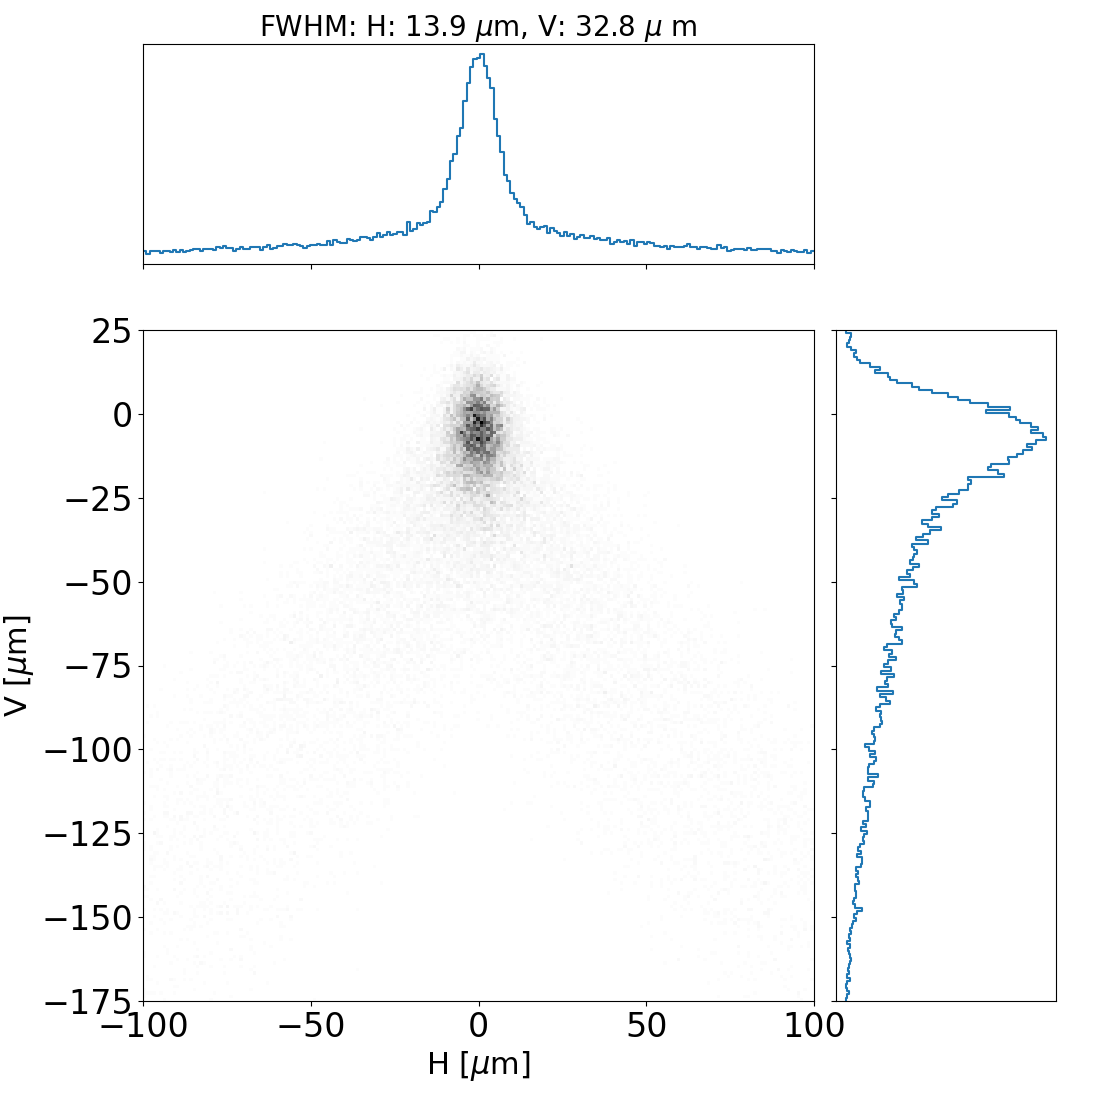
\includegraphics[width=0.49\textwidth]{figures/prefinal_approx1_linearized.png}\\
% 
% \flushleft
% c)~~~~~~~~~~~~~~~~~~~~~~~~~~~~~~~~~~~~~~~~~~~~~~~~~d)\\
% \centering
% 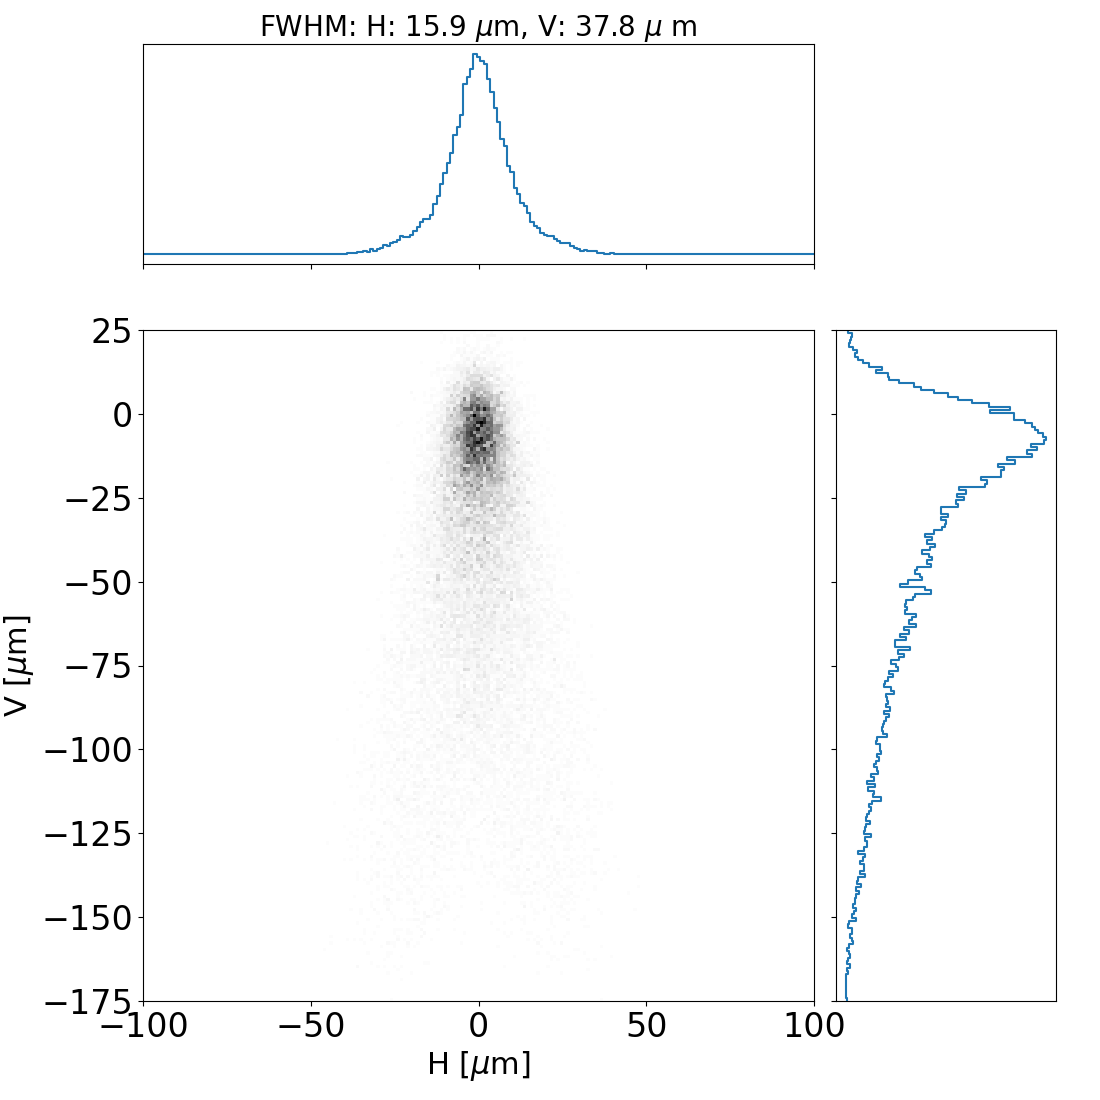
\includegraphics[width=0.49\textwidth]{figures/prefinal_approx2.png} 
% 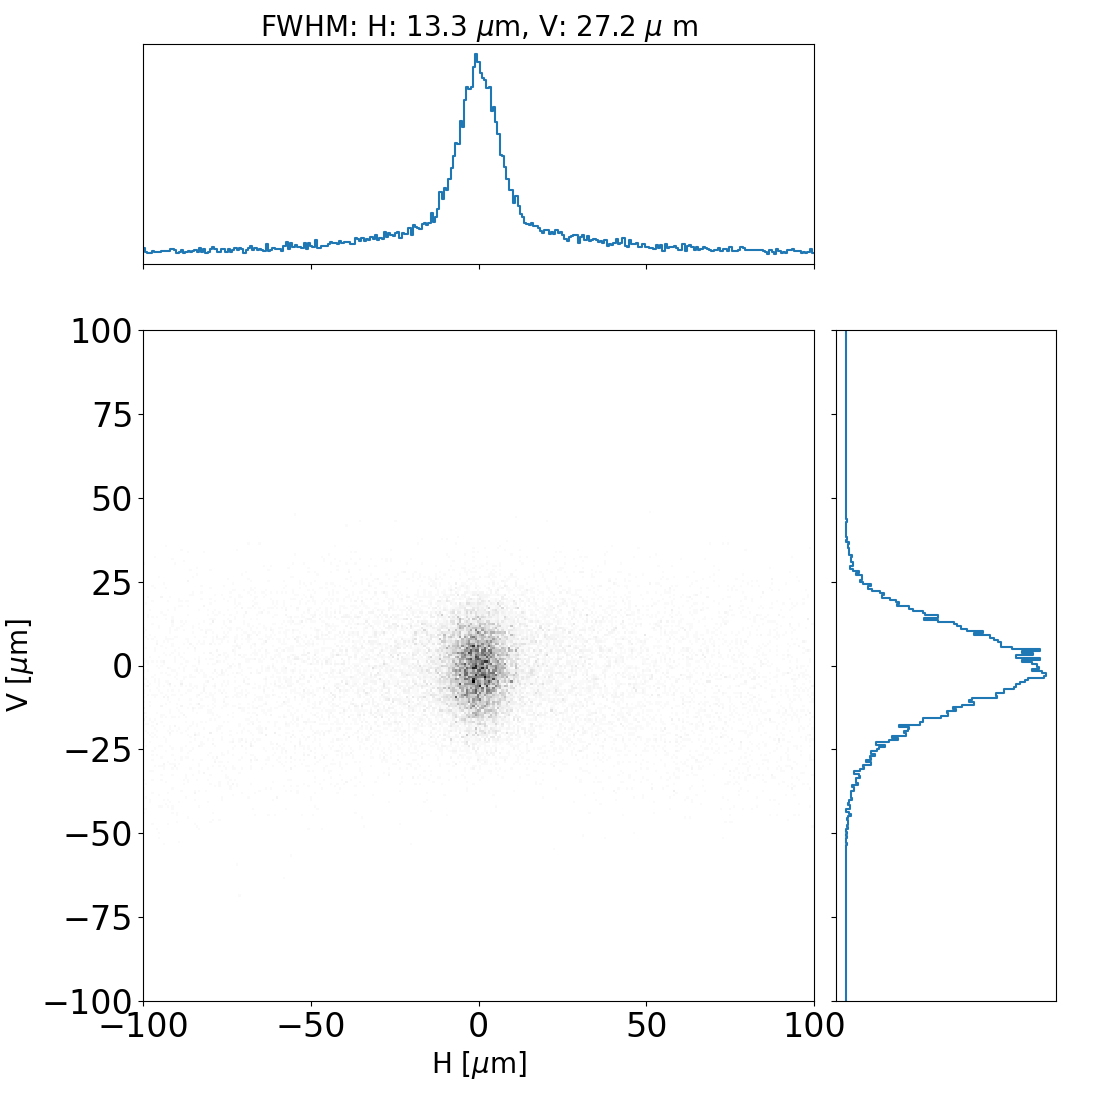
\includegraphics[width=0.49\textwidth]{figures/prefinal_approx1_exact1over2.png} 


\caption{Calculated focal spots produced by ALS Beamline 12.2.2 with the diaboloid approximated by four surfaces: (\textbf{a}) a cone (\inred{sagittal linearly varying} circular section) bent to a parabola \inred{in the tangential direction}, (\textbf{b}) a cylinder (\inred{ sagittal uniform} circular section) bent to a parabola in the tangential direction, (\textbf{c}) a cylinder (\inred{sagittal uniform} elliptical section) bent to a parabola \inred{in the tangential direction}, and (\textbf{d}) like (\textbf{b}) but in the exact 1:2 configuration ($M$~= $q$:$p$ = 9.4:18.8).
\inred{For comparison, the exact diaboloid gives a spot size of 10 $\times$~\SI{18}{\micro\meter}$^2$ (Fig.~\ref{fig:als}b$_2$).}
}
\end{figure}

\section{Summary}
\label{sec:summary}

The diaboloid is a hybrid optical surface that focuses light from infinity to a point in one direction, and in the orthogonal direction, focuses from a real source to a stigmatic point. To date, toroidal mirrors have served this purpose on x-ray beamlines, but as source sizes decrease, the residual aberrations become significant. With the advent of diffraction limited storage rings with very bright bending magnet sources, there is a need for better focusing. 

The diaboloid provides aberration-free focusing and will be useful in all cases where there is a vertically collimating pre-mirror, as is common \inred{in beamlines using a bending magnet (or a short wiggler) source} and a double-crystal monochromator. The optimal shape departs from more commonly used optical surfaces, but at 1:2 horizontal magnification, the shape comes closest to a toroid, bringing it within reach of current manufacturing.
%devolves to parabolic curvature in the tangential direction and elliptical curvature in the sagittal direction.
For \SI{5}{\milli\radian} grazing angles, and typical beamline parameters, the deviation of the surface from toroidal is below \SI{2}{\micro\meter}, a thickness at which sputtering can be used to deposit a thin, spatially-graded, correcting layer. Additionally, at the 1:2 magnification condition, the parabolic tangential shape could be created by bending, and the unbent mirror would have elliptical or circular sagittal cross-sections. This opens up possibilities for normal-incidence optical interferometry.

As fabrication and metrology improve, diaboloids can be used to produce aberration-free focusing under any magnification, exceeding the performance of toroids and offering the possibility of \inred{simplifying the} beamlines by eliminating the need for additional demagnifying elements. \inred{The Oasys workspace containing the optical systems discussed in this work and other support files are available at the address: \url{https://github.com/oasys-als-kit/Paper\_JSR\_hf5419}}


   %-------------------------------------------------------------------------
   % The back matter of the paper - acknowledgements and references
   %-------------------------------------------------------------------------

   % Acknowledgements come after the appendices

\vspace{5mm}
\section{Acknowledgements}    
 
We acknowledge Wayne McKinney for valuable discussions and insight.
This work was supported by the Director, Office of Science, Office of Basic Energy Sciences, of the U.S. Department of Energy under Contract No. DE-AC02-05CH11231.

\appendix

\section{The explicit form of the diaboloid }
\label{appendix:diaboloid}

Using the schematic view in Fig.~\ref{fig:frame}, in the plane of incidence, the distance from the source $(0,-p,0)$ to the image $(0,q \cos2\theta, q \sin2\theta)$, passing through the mirror pole $(0,0,0)$ is $p+q$. In this orientation, the incident light cone is centered on the $y$-axis. By Fermat's principle, this distance must be the same when passing through any point $(x,y,z)$ of the mirror surface to a corresponding point on the line-image:

% https://www.wolframalpha.com/input/?i=Solve%5Bsqrt%28x%5E2%2B%28y%2Bp%29%5E2%29+%2B+sqrt%28x%5E2%2B%28q+cos%282t%29-y%29%5E2+%2B+%28q+sin%282t%29-z%29%5E2%29-%28p%2Bq%29%3D0%3Bz%5D
\begin{multline}
\label{eqn:distances}
p + q = 
\sqrt{x^2 + (y + p)^2} + \\
\sqrt{x^2 + (q \cos2 \theta - y)^2 + (q \sin2 \theta - z)^2}.
\end{multline}
This equation can be solved exactly, obtaining equation~(\ref{eqn:diaboloidV}), that determines the mirror height $z$ for every point $(x,y)$ on the surface.
%\begin{multline}
%\label{eqn:explicit}
%z = q \sin2\theta - 
%[-2 (p + q) \sqrt{p^2 + 2 p y + x^2 + y^2} + \\ 
%2 p^2 +2 p q + 2 p y - q^2 cos^2 2 \theta + q^2 + 2 q y \cos2\theta %]^{1/2},
%\end{multline}
%which is the same as Eq.~\ref{eqn:diaboloidV}. 

In the $yz$ plane, With $x$~= 0, the tangential section is a parabola. The equation of the parabola with axis of symmetry parallel to the $y$ axis (Fig.~\ref{fig:frame}) can be written 
\begin{equation}
y = -\frac{z^2}{4 f} + \frac{v_z z}{2 f} - \left(\frac{v_z^2}{4 f} + v_y\right),
\end{equation}
\noindent with focal distance $f$ and vertex $(v_y,v_z)$. Developing equation~(\ref{eqn:distances}) for $x=0$ and matching coefficients we find $f=(1-\cos2\theta)q/2$, $v_z=q \sin2\theta$ and $v_y=f+q\cos2\theta$.

The sagittal section is approximately an ellipse. For $y=0$ in equation~(\ref{eqn:diaboloidV}) we have

\begin{multline}
\label{eqn:ellipse2}
(z - q \sin2\theta)^2 = \\
-2 (p + q) \sqrt{p^2 + x^2}+ 
2 p^2 +2 p q + q^2 \sin^2 2 \theta.
\end{multline}
Expanding the square root for $x\ll p$, we obtain the ellipse equation
\begin{equation}
\label{eqn:ellipse}
\frac{x^2}{a_x^2} + \frac{(z-q \sin2\theta)^2}{a_z^2}=1
\end{equation}
with semiaxes $a_z=q \sin2\theta$ and $a_x=a_z\sqrt{q/(p+q)}$.


   % References are at the end of the document, between \begin{references}
   % and \end{references} tags. Each reference is in a \reference entry.

% \begin{references}
% \reference{Author, A. \& Author, B. (1984). \emph{Journal} \textbf{Vol}, 
% first page--last page.}
% \end{references}
%\cite{knuth84}

%% Note added by Overleaf: If using bibtex, remove the "references" environment above, and uncomment the following line.
\referencelist{iucr}


%   %-------------------------------------------------------------------------
%   % TABLES AND FIGURES SHOULD BE INSERTED AFTER THE MAIN BODY OF THE TEXT
%   %-------------------------------------------------------------------------
% 
%   % Simple tables should use the tabular environment according to this
%   % model
% 
% \begin{table}
% \caption{Caption to table}
% \begin{tabular}{llcr}   % Alignment for each cell: l=left, c=center, r=right
% HEADING  & FOR    & EACH    & COLUMN   \\
% \hline
% entry   & entry   & entry   & entry   \\
% entry   & entry   & entry   & entry   \\
% entry   & entry   & entry   & entry   \\
% \end{tabular}
% \end{table}
% 
%   % Postscript figures can be included with multiple figure blocks
% 
% \begin{figure}
% \caption{Caption describing figure.}
% \includegraphics{fig1}
% \end{figure}


\end{document}          % DO NOT DELETE THIS LINE
%%%%%%%%%%%%%%%%%%%%%%%%%%%%%%%%%%%%%%%%%%%%%%%%%%%%%%%%%%%%%%%%%%%%%%%%%%%%%%


